%%
%% Anonymous ACM submission
%%
\documentclass[sigconf,balance=false]{acmart}

\AtBeginDocument{%
  \providecommand\BibTeX{{Bib\TeX}}}

\setcopyright{none}
\settopmatter{printacmref=true}
\acmYear{2026}
\acmConference[Anonymous Submission]{Anonymous Submission}{2026}{Venue withheld for review}
\acmBooktitle{Anonymous Submission}
\acmDOI{}
\acmISBN{}

\usepackage{hyperref}
\usepackage{url}
\usepackage{booktabs}
\usepackage{amsfonts}
\usepackage{amsmath}
\usepackage{bm}
\usepackage{algorithm}
\usepackage{algpseudocode}
\usepackage{graphicx}
\usepackage{enumitem}
\usepackage{placeins}
\usepackage{balance}
\usepackage{microtype}
\usepackage{xcolor}
\usepackage{tikz}
\usetikzlibrary{arrows.meta,backgrounds,calc,fit,positioning}

\definecolor{cimTeal}{HTML}{1F6F78}
\definecolor{cimGold}{HTML}{C28B2C}
\definecolor{cimRed}{HTML}{A95050}
\definecolor{cimBlue}{HTML}{496F9B}
\definecolor{cimGray}{HTML}{667078}
\definecolor{cimLight}{HTML}{F3F5F5}
\tikzset{
  cimnode/.style={circle,draw=cimGray,fill=white,minimum size=5.8mm,
                  inner sep=0pt,font=\scriptsize},
  cimseed/.style={cimnode,draw=cimBlue,very thick,fill=cimBlue!10},
  cimadopt/.style={cimnode,draw=cimTeal,very thick,fill=cimTeal!13},
  cimdrop/.style={cimnode,draw=cimRed,very thick,fill=cimRed!10},
  cimset/.style={rounded corners=2pt,draw=cimGray,fill=cimLight,
                 inner xsep=5pt,inner ysep=4pt,font=\scriptsize},
  cimarrow/.style={-{Latex[length=2mm]},semithick,cimGray},
  cimlabel/.style={font=\scriptsize,align=center}
}

\newcommand{\CIMRIS}{\textsc{CIM-RIS}}
\newcommand{\E}{\mathbb{E}}
\newcommand{\I}{\mathbb{I}}

\begin{document}

\title{Coupon Influence Maximization under Non-Replicable Diffusion}

\author{Anonymous Author(s)}

\renewcommand{\shortauthors}{Anon.}

%% ============================================================
%% ABSTRACT
%% ============================================================
\begin{abstract}
Classical influence maximization assumes copyable information that can
branch from one activated user to multiple neighbors.
Digital coupons instead move as non-replicable objects: a recipient
redeems, discards, or forwards a coupon to one neighbor, and only
redemption creates an adopter.
We formalize this setting as coupon influence maximization (CIM), which
allocates a limited number of independently diffusing coupons to maximize
the expected number of distinct adopters.
We prove that CIM is NP-hard and show that adoption spread is monotone
and has diminishing returns over integer coupon allocations.
Exact greedy consequently achieves a $(1-1/e)$ approximation, but its
marginal gains are expensive to evaluate.
We therefore develop $k$-joint reverse reachable samples that preserve
coupon identities and separate root adoption from reverse reachability.
The resulting coverage events yield unbiased estimators of spread and
marginal gain.
Based on these estimators, \CIMRIS{} returns a
$(1-1/e-\epsilon)$-approximate allocation with high probability and runs
in expected near-linear time in the graph size when the budget, accuracy,
and spread lower bound are fixed.
Experiments on five graph instances derived from real networks show
competitive solution quality and practical scalability. Across two graphs
and three scenarios with high-precision Monte Carlo greedy references, the
observed gap is $0.3$--$11.1\%$; on Netscience, it is $1.1$--$4.4\%$.
\CIMRIS{} outperforms both degree and PageRank baselines in all 72
graph--scenario--budget configurations, while
conditioned root sampling improves the variance--time product by
$1.3\times$ and $1.5\times$ at $k=10$ on Netscience and EmailEnron.
\end{abstract}

\begin{CCSXML}
<ccs2012>
 <concept>
  <concept_id>10002951.10002952.10002953.10010820</concept_id>
  <concept_desc>Information systems~Social networks</concept_desc>
  <concept_significance>500</concept_significance>
 </concept>
 <concept>
  <concept_id>10003752.10003809.10010170.10010171</concept_id>
  <concept_desc>Theory of computation~Approximation algorithms analysis</concept_desc>
  <concept_significance>300</concept_significance>
 </concept>
</ccs2012>
\end{CCSXML}

\ccsdesc[500]{Information systems~Social networks}
\ccsdesc[300]{Theory of computation~Approximation algorithms analysis}

\keywords{influence maximization, coupon diffusion, random walk,
          reverse influence sampling, submodular optimization}

\maketitle

\hypersetup{
  pdftitle={Coupon Influence Maximization under Non-Replicable Diffusion},
  pdfauthor={Anonymous Author(s)},
  pdfkeywords={influence maximization, coupon diffusion, random walk,
    reverse influence sampling, submodular optimization}
}

%% ============================================================
%% 1. INTRODUCTION
%% ============================================================
\section{Introduction}
\label{sec:intro}

Word-of-mouth and viral marketing are important strategies for promoting
product adoption in online social networks.
Influence maximization (IM) asks how to select a limited number of seed
users whose diffusion activates as many users as possible~\cite{kempe2003maximizing}.
Over the past two decades, IM has been extensively studied under the
Independent Cascade (IC) and Linear Threshold (LT) models, where an
activated user may influence multiple neighbors and thereby create a
branching cascade~\cite{domingos2001mining,borgs2014maximizing,tang2015influence}.
Many promotional objects, however, are non-replicable and cannot be
described by this broadcast assumption.
A digital coupon, for example, can be redeemed, discarded, or forwarded
to one friend, but it cannot be simultaneously copied to many neighbors.
Its diffusion is therefore a random-walk-like path rather than a cascade.

Consider a company that distributes $k$ digital coupons through a social
network.
When a user receives a coupon, the user may redeem it, discard it, or
forward it to one out-neighbor.
Redemption and discard both terminate the coupon, whereas forwarding
moves the same coupon to the next user without creating another copy.
A user is counted as an adopter only after redeeming at least one coupon;
users who merely forward coupons do not contribute to the campaign
objective.
Different coupons diffuse independently, and several coupons may be
redeemed by the same user, but that user is counted only once.
The company may also assign multiple coupons to the same initial user,
since independent coupons starting from that user can follow different
paths.

These dynamics raise a seed-allocation problem that is distinct from
classical IM.
Placing many coupons at individually strong seeds may cause their
trajectories to overlap at the same adopters, while placing coupons at
poor seeds may result in excessive discards.
We therefore define \emph{coupon influence maximization} (CIM): given a
budget of $k$ coupons, allocate them to seed users so as to maximize the
expected number of distinct adopters.
We also consider coupon usage rate, the expected fraction of issued
coupons that are eventually redeemed, as a complementary campaign
measure.

We formalize the coupon diffusion process and establish the computational
and structural properties of CIM.
We prove that CIM is NP-hard and show that its adoption-spread objective
has diminishing returns over coupon allocations.
This property suggests a greedy allocation strategy, but direct marginal
evaluation by forward Monte Carlo simulation is too expensive for large
networks.
Inspired by reverse influence sampling (RIS), we construct coupon-aware
reverse reachable (RR) samples and convert marginal evaluation into a
coverage computation.
The resulting \CIMRIS{} algorithm achieves a
$(1-1/e-\epsilon)$ approximation with high probability.

CIM differs from classical IM at both the model and algorithmic levels.
In IC and LT, activation and propagation are coupled: an activated user
may continue the cascade through multiple neighbors.
In CIM, propagation follows one forwarding path, and an intermediate
forwarder remains a non-adopter.
Algorithmically, a classical RR set represents one broadcast realization,
whereas a CIM sample must preserve the independent realization and
identity of every coupon.
Consequently, neither classical RR-set generation nor its induced
maximum-coverage procedure can be applied directly.

In summary, our contributions are threefold.
First, we introduce the coupon influence model and formally define CIM,
capturing non-replicable single-path diffusion, independent coupons, and
overlap among adopters.
Second, we prove the NP-hardness of CIM and establish the diminishing-return
property of its adoption spread over integer coupon allocations, which
supports a $(1-1/e)$ greedy approximation when marginal gains are exact.
Third, we develop coupon-aware RR sampling and the scalable \CIMRIS{}
algorithm, which estimates these marginal gains and retains a
$(1-1/e-\epsilon)$ approximation guarantee with high probability.
Experiments on five graph instances derived from real networks evaluate its
solution quality, scalability, sensitivity to the sampling budget,
capacity-aware placement, and the variance reduction obtained by conditioned
root sampling. In particular, \CIMRIS{} is competitive with Monte Carlo
greedy, consistently improves over topology-only seed rankings, and selects
200 seeds on the 154,907-node Douban instance in 31.2 seconds using the
validated sample budget.


%% ============================================================
%% 2. RELATED WORK
%% ============================================================
\section{Related Work}
\label{sec:related}

\textbf{Influence maximization.}
Early studies established viral marketing as an optimization problem
over social networks~\cite{domingos2001mining,richardson2002mining}.
Kempe et al.~\cite{kempe2003maximizing} formalized IM under the IC and
LT models, proved NP-hardness, and used monotonicity and submodularity to
obtain a $(1-1/e)$ greedy approximation.
Subsequent work accelerated marginal evaluation through lazy greedy
methods and model-specific optimizations
~\cite{leskovec2007celf,goyal2011celf,chen2009efficient}.
These models describe copyable influence: an activated node can attempt
to activate several neighbors.
CIM instead allocates non-replicable coupons, each of which follows one
forwarding path and creates an adopter only when a user redeems it.

\textbf{Reverse influence sampling.}
Borgs et al.~\cite{borgs2014maximizing} introduced the RR-set approach
that converts influence estimation into random-set coverage.
TIM/TIM+~\cite{tang2014influence}, IMM~\cite{tang2015influence},
Stop-and-Stare~\cite{nguyen2016stop,huang2017revisiting}, and
OPIM-C~\cite{tang2018online} progressively improved the theoretical and
practical efficiency of this framework.
Their fundamental coverage event is that a seed set intersects one RR
set generated from a broadcast realization.
Our reverse construction differs in two ways: adoption at the root is a
separate gate, and one sample contains independent RR components for the
individual coupons.
This indexed construction is necessary to estimate the distinct adopters
created by a coupon allocation.

\textbf{Diffusion variants.}
IM has also been studied under competitive diffusion, misinformation
control, location constraints, adaptive seeding, and multi-round
campaigns
~\cite{budak2011limiting,li2014efficient,lu2015competition,seeman2013adaptive,sun2018multi}.
Most directly related to our application, Liao et
al.~\cite{liao2023popularity} use coupon distribution as the motivation
for allocating promotional seeds across rounds to improve a product's
popularity ratio.
Their PA-IC model nevertheless propagates copyable promotional
information through an IC cascade; it does not model each coupon as the
single object being forwarded and consumed.
Random-walk processes provide a classical foundation for single-path
movement on graphs~\cite{lovasz1993random}, but standard random-walk
objectives do not capture the combination of terminal adoption,
non-replicability, and overlap among independently issued coupons.
CIM brings these features into one optimization model and develops a
coupon-aware reverse sampler for it.

%% ============================================================
%% 3. MODEL AND PROBLEM DEFINITION
%% ============================================================
\section{Model and Problem Definition}
\label{sec:model}

This section introduces the coupon influence model, which combines
non-replicable coupons with single-path, random-walk-like propagation in a
social network. We then formulate Coupon Influence Maximization (CIM), which
allocates $k$ coupons to initial recipients to maximize the expected number of
distinct adopters.

\subsection{Coupon Influence Model}

Classical IM is commonly studied under the Independent Cascade (IC) and
Linear Threshold (LT) models~\cite{kempe2003maximizing}.
At time step $0$, all seed nodes are activated and the remaining nodes
are inactive; once activated, a node remains activated.
Under IC, a node activated at time step $i$ has one chance to activate
each inactive out-neighbor at time step $i+1$, independently according
to the propagation probability on the connecting edge.
Under LT, each node independently selects a threshold from $[0,1]$ and
becomes activated once the total weight from its activated in-neighbors
reaches that threshold.
The propagation terminates when no more nodes can be activated.
Scalable IM algorithms typically solve this problem using reverse
influence sampling (RIS)~\cite{borgs2014maximizing,tang2015influence}.
A random reverse reachable (RR) set is generated by first sampling a root
node uniformly from $V$ and then tracing backward all nodes that can
activate the root in a random diffusion realization.
For any seed set $S$, its expected influence equals
$n\Pr[S\cap R\neq\emptyset]$; hence, IM can be transformed into a maximum
coverage problem over sampled RR sets.
Given $\theta$ independent RR sets, the fraction covered by $S$ gives
both the maximum-likelihood estimate and an unbiased estimate of its
normalized influence.
The required value of $\theta$ is determined adaptively using an
estimated lower bound on the optimal influence together with
concentration bounds, after which a greedy algorithm selects the $k$
nodes with the largest marginal RR-set coverage.
CIM follows the same high-level optimization route, but its single-path,
non-replicable coupon diffusion requires a different RR-set generation
process and a different induced coverage problem.

We model the social network as a directed graph $G=(V,E)$, where $V$ is
the set of $n=|V|$ users and $E$ is the set of $m=|E|$ directed
forwarding relationships.
Let $V_s\subseteq V$ be the set of eligible seed users; we use $V_s=V$
when every user is eligible.
Each $v\in V_s$ has a placement capacity $c_v\in\{1,\ldots,k\}$.
Setting $c_v=1$ requires distinct seeds, while $c_v=k$ permits all
coupons to be assigned to the same user.
We assume $\sum_{v\in V_s}c_v\geq k$.
Each node $u\in V$ has an adoption probability $p_u^a$, a discard
probability $p_u^d$, and a transfer probability $p_u^t$, where
$p_u^a+p_u^d+p_u^t=1$.
For every edge $(u,v)\in E$, $p(u,v)$ denotes the unconditional
probability that $u$ transfers its coupon to $v$; accordingly,
$\sum_{v:(u,v)\in E}p(u,v)=p_u^t$.
For a node with no out-neighbor, we require $p_u^t=0$.

Consider one coupon seeded at $s\in V_s$.
At time step $0$, node $s$ holds the coupon.
If node $u$ holds it at time step $\tau$, then $u$ redeems the coupon and
becomes an adopter with probability $p_u^a$, or discards it with
probability $p_u^d$; either action terminates this coupon's diffusion.
Otherwise, $u$ transfers the coupon to out-neighbor $v$ with probability
$p(u,v)$, and $v$ holds it at time step $\tau+1$.
Thus, a coupon generates one forwarding path rather than a branching
cascade.

Propagation and adoption are separate in this process.
A forwarding user may help the coupon reach a later adopter without
becoming an adopter, while a user contributes to the objective only by
redeeming the coupon.
This separation is absent from classical IC and LT diffusion, where an
activated node can continue propagating influence.

We use a realization-space view to analyze the random process.
For every coupon $j\in[k]$, an independent realization $W_j$ fixes the
action taken by every node for that coupon.
Specifically, for each node $u\in V$ and coupon $j$, we draw an
independent random number $r_{u,j}\sim\mathrm{Uniform}[0,1]$.
We use this number to choose the action of $u$ by partitioning the unit
interval into one adoption segment of length $p_u^a$, one discard
segment of length $p_u^d$, and one transfer segment for each
out-neighbor $v$, whose length is $p(u,v)$.
Let $\Phi_j(u)$ denote the resulting action of $u$ in realization $W_j$.
Then $\Phi_j(u)=\textsf{adopt}$ means that $u$ redeems coupon $j$,
$\Phi_j(u)=\textsf{discard}$ means that $u$ discards it, and
$\Phi_j(u)=v$ means that $u$ transfers it to out-neighbor $v$.
The collection $W_j=\{r_{u,j}\}_{u\in V}$ is the realization of coupon
$j$, and $\mathcal{W}=(W_1,\ldots,W_k)$ fully determines the outcome of
all coupons.

Under this construction, coupon $j$ seeded at $s_j$ is redeemed by node $u$
if and only if it reaches $u$ under realization $W_j$ and $u$ takes the
adoption action in that realization.
Let $A_{u,j}$ denote the event $r_{u,j}\leq p_u^a$.
We write
\[
  \mathrm{Adopt}_{u,j}(s_j)
  = A_{u,j}\wedge
    \{\text{coupon }j\text{ starting from }s_j
      \text{ reaches }u\text{ in }W_j\}.
\]
Here $A_{u,j}$ depends on the action of the target node, whereas the
reachability event depends on the actions of preceding nodes on the
forwarding path.
The construction therefore separates reaching a user from adoption by
that user.

For a campaign with $k$ coupons, let $S=(s_1,\ldots,s_k)$ be an ordered
seed tuple, where coupon $j$ starts from $s_j$.
The coupons diffuse independently and do not block or modify one another.
Each coupon follows its own path until it is redeemed, discarded, or
trapped in a transfer cycle.
Different coupons may reach the same user, who may redeem more than one of
them; that user contributes one adopter to the objective regardless of the
number of coupons redeemed.
Consequently, the coupons are independent at the diffusion level but
coupled through distinct-user coverage in the campaign objective.

For a seed tuple $S=(s_1,\ldots,s_k)$, node $u$ becomes an adopter if
\[
  \mathrm{Adopt}_u(S) = \bigvee_{j=1}^{k} \mathrm{Adopt}_{u,j}(s_j).
\]

\begin{figure*}[t]
  \centering
  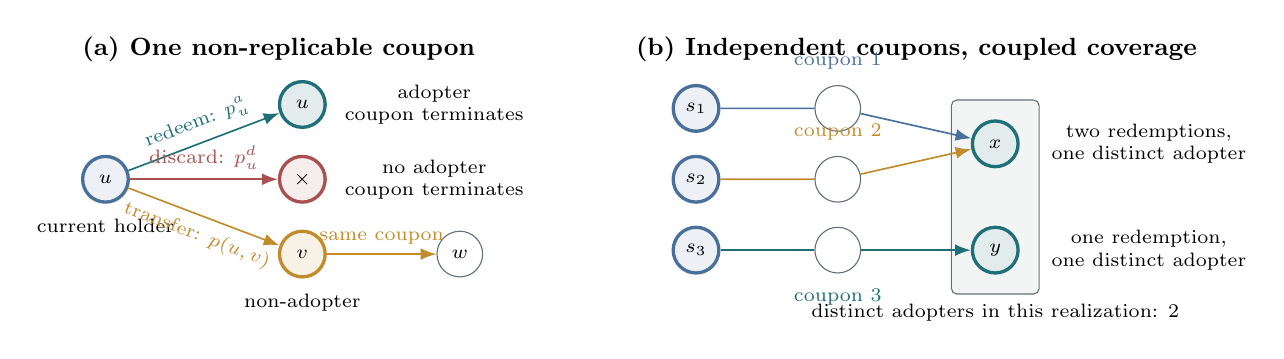
\begin{tikzpicture}[x=1cm,y=1cm]
    \begin{scope}
      \node[cimlabel,font=\small\bfseries] at (2.7,1.65)
        {(a) One non-replicable coupon};
      \node[cimseed] (u) at (0.5,0) {$u$};
      \node[cimlabel,below=2pt of u] {current holder};
      \node[cimadopt] (a) at (3.0,0.95) {$u$};
      \node[cimdrop] (d) at (3.0,0) {$\times$};
      \node[cimnode,draw=cimGold,very thick,fill=cimGold!12]
        (v) at (3.0,-0.95) {$v$};
      \node[cimnode] (w) at (5.0,-0.95) {$w$};
      \draw[cimarrow,cimTeal] (u) -- node[above,sloped,cimlabel]
        {redeem: $p_u^a$} (a);
      \draw[cimarrow,cimRed] (u) -- node[above,cimlabel]
        {discard: $p_u^d$} (d);
      \draw[cimarrow,cimGold] (u) -- node[below,sloped,cimlabel]
        {transfer: $p(u,v)$} (v);
      \draw[cimarrow,cimGold] (v) -- node[above,cimlabel]
        {same coupon} (w);
      \node[cimlabel,right=3pt of a] {adopter\\coupon terminates};
      \node[cimlabel,right=3pt of d] {no adopter\\coupon terminates};
      \node[cimlabel,below=2pt of v] {non-adopter};
    \end{scope}

    \begin{scope}[xshift=8.0cm]
      \node[cimlabel,font=\small\bfseries] at (2.8,1.65)
        {(b) Independent coupons, coupled coverage};
      \node[cimseed] (s1) at (0,0.9) {$s_1$};
      \node[cimseed] (s2) at (0,0) {$s_2$};
      \node[cimseed] (s3) at (0,-0.9) {$s_3$};
      \node[cimnode] (m1) at (1.8,0.9) {};
      \node[cimnode] (m2) at (1.8,0) {};
      \node[cimnode] (m3) at (1.8,-0.9) {};
      \node[cimadopt] (x) at (3.8,0.45) {$x$};
      \node[cimadopt] (y) at (3.8,-0.9) {$y$};
      \draw[-{Latex[length=2mm]},semithick,cimBlue]
        (s1) -- (m1) -- (x);
      \draw[-{Latex[length=2mm]},semithick,cimGold]
        (s2) -- (m2) -- (x);
      \draw[-{Latex[length=2mm]},semithick,cimTeal]
        (s3) -- (m3) -- (y);
      \node[cimlabel,above=2pt of m1,text=cimBlue] {coupon 1};
      \node[cimlabel,above=2pt of m2,text=cimGold] {coupon 2};
      \node[cimlabel,below=2pt of m3,text=cimTeal] {coupon 3};
      \node[cimlabel,right=8pt of x] {two redemptions,\\one distinct adopter};
      \node[cimlabel,right=8pt of y] {one redemption,\\one distinct adopter};
      \begin{scope}[on background layer]
        \node[cimset,fit=(x)(y),inner sep=7pt,
              label={[cimlabel]below:distinct adopters in this realization: $2$}] {};
      \end{scope}
    \end{scope}
  \end{tikzpicture}
  \caption{Coupon diffusion and multi-coupon overlap.
  Redemption and discard terminate a coupon, whereas transfer moves the
  same coupon to one neighbor.
  Coupons diffuse independently, but multiple redemptions by the same
  user contribute only one distinct adopter.}
  \Description{Two panels illustrate coupon diffusion. The first shows
  redeem, discard, and one-neighbor transfer outcomes. The second shows
  three independent coupons ending at two distinct adopters.}
  \label{fig:model-overview}
\end{figure*}

\textbf{Comparison and boundary cases.}
The coupon model differs from related diffusion and simulation settings
in three respects.
\begin{itemize}
  \item \emph{Classical influence maximization.}
  IC and LT diffusion models describe copyable influence: once a user is
  activated, the influence attempt may branch to multiple neighbors.
  In CIM, each coupon is non-replicable and moves to at most one
  out-neighbor at each step, so the diffusion trace of one coupon is a
  path rather than a cascade.

  \item \emph{Forward Monte Carlo evaluation.}
  Forward Monte Carlo simulation can estimate the adoption spread of a
  fixed seed tuple by sampling coupon trajectories.
  Optimization, however, requires repeated marginal evaluation over many
  allocations, making direct simulation expensive.

  \item \emph{Repeated visits and coupon overlap.}
  The realization-space view fixes the behavior of each node for each
  coupon.
  Therefore, if the same coupon revisits a node through transfer actions,
  it follows a deterministic transfer cycle and contributes no adoption
  in that realization.
  Different coupons use independent realizations and may be redeemed by
  the same user, but the adoption spread counts that user only once.
\end{itemize}

\textbf{Challenge.}
The central algorithmic challenge is to estimate marginal gains without
repeated forward simulations while preserving independent coupon
realizations and distinct-user coverage.

\subsection{Problem Formulation}

For an ordered seed tuple $S=(s_1,\ldots,s_k)\in V_s^k$, define its
allocation vector $\bm{x}(S)\in\mathbb{Z}_{\geq 0}^{V_s}$ by
$x_v(S)=|\{j:s_j=v\}|$.
Thus $\sum_{v\in V_s}x_v(S)=k$; repeated seed nodes are allowed whenever
their capacities exceed one.
Feasible allocations also satisfy $x_v\leq c_v$.
Because coupons diffuse independently according to the same model, the
expected outcome depends on $S$ only through $\bm{x}(S)$.

We define the adoption spread as the expected number of distinct users who
redeem at least one coupon:
\[
  \sigma(S) = \sum_{u \in V}
    \Pr\!\left[\mathrm{Adopt}_u(S)\right]
  = \sum_{u \in V}
    \Pr\!\left[\bigvee_{j=1}^{k} \mathrm{Adopt}_{u,j}(s_j)\right].
\]
For nodes $v,u\in V$, let $q_{vu}$ be the probability that one coupon
seeded at $v$ is eventually redeemed by $u$.
Independence among coupons gives the equivalent allocation form
\[
  \sigma(\bm{x})=
  \sum_{u\in V}\left(1-\prod_{v\in V_s}(1-q_{vu})^{x_v}\right).
\]
The product is the probability that none of the allocated coupons is redeemed
by $u$.
This form makes explicit that each adopter is counted once.

We also define the expected total number of redeemed coupons as
\[
  \rho(S) =
  \sum_{j=1}^{k}
    \Pr\!\left[\bigvee_{u\in V} \mathrm{Adopt}_{u,j}(s_j)\right],
\]
where the inner event means that coupon $j$ is eventually redeemed by
some user.
Since each coupon can be redeemed at most once, $0\leq\rho(S)\leq k$.
Equivalently,
\[
  \rho(\bm{x})=\sum_{v\in V_s}x_v\sum_{u\in V}q_{vu}.
\]
The corresponding coupon usage rate is
\[
  \eta(S)=\frac{\rho(S)}{k},
  \qquad
  \eta(\bm{x})=\frac{\rho(\bm{x})}{k}.
\]
The two quantities capture different goals: $\sigma$ emphasizes distinct
adopters, whereas $\eta$ emphasizes coupon utilization.

\begin{definition}[CIM: Adoption-Spread Maximization]
\label{def:cim}
Given (a) a directed social network $G=(V,E)$, (b) an eligible seed set
$V_s\subseteq V$ with capacities $\bm{c}$, (c) node behavior parameters
$\{(p_u^a,p_u^d,p_u^t)\}_{u\in V}$, (d) edge forwarding parameters
$\{p(u,v)\}_{(u,v)\in E}$, and (e) a coupon budget $k$, the
task of Coupon Influence Maximization (CIM) is to find a coupon allocation
$\bm{x}^*$ of total size $k$ that maximizes adoption spread:
\[
  \bm{x}^*=\arg\max_{\substack{\bm{x}\in\mathbb{Z}_{\geq0}^{V_s}\\
  \|\bm{x}\|_1=k,\ \bm{x}\leq\bm{c}}}\sigma(\bm{x}).
\]
\end{definition}

\begin{definition}[Coupon Usage-Rate Maximization]
\label{def:usage-rate}
Given the same input as in Definition~\ref{def:cim}, coupon usage-rate
maximization seeks an allocation $\bm{x}^\dagger$ that
maximizes the expected coupon usage rate:
\[
  \bm{x}^\dagger =
  \arg\max_{\substack{\bm{x}\in\mathbb{Z}_{\geq0}^{V_s}\\
  \|\bm{x}\|_1=k,\ \bm{x}\leq\bm{c}}}
  \eta(\bm{x}).
\]
\end{definition}

In this paper, CIM refers to the adoption-spread maximization problem
unless otherwise stated.
The usage-rate objective is a complementary objective that is useful
when the campaign organizer mainly cares about how many issued coupons are
redeemed.
Because $\rho(\bm{x})$ is linear in $\bm{x}$, usage-rate maximization
fills seed capacities in descending order of the single-coupon redemption
probability $\sum_u q_{vu}$.
In contrast, $\sigma(\bm{x})$ penalizes overlap at the same adopters and
therefore creates a non-trivial allocation problem.

For adoption spread, assigning every coupon to its individually best seed may
be suboptimal because several coupons may end at the same adopter, who is
counted only once in $\sigma(S)$. Conversely, graph distance alone is
insufficient: a distant seed with a low probability of reaching an adopter may
contribute little. CIM must therefore balance path-based reachability against
overlap among the adopters reached by different coupons.
Section~\ref{sec:algo} uses an ordered tuple only to associate each
allocated coupon with an independent RR component; any ordering of the
same allocation vector has the same expected spread.

For example, consider two independent realizations: coupon~1 is
seeded at $s_1$ in realization $W_1$, and coupon~2 is seeded at $s_2$ in
realization $W_2$.
In realization $W_1$, the forwarding path from $s_1$ reaches node $u$, and
the adoption event $A_{u,1}$ occurs, so $u$ redeems coupon~1 and becomes an
adopter.
In realization $W_2$, coupon~2 follows a different forwarding path and
is redeemed by node $v$.
Node $w$ lies on the forwarding chains but does not redeem either coupon; it
helps propagation but does not contribute to the objective.
Therefore, in this realization, the number of adopters is two.

%% ============================================================
%% 4. THEORETICAL ANALYSIS
%% ============================================================
\section{Theoretical Analysis}
\label{sec:theory}

We first prove that CIM is NP-hard, even on a two-layer diffusion graph.
We then show that adoption spread is monotone and has diminishing returns
over integer coupon allocations.
This structure yields a $(1-1/e)$ approximation for exact greedy, but
computing its marginal gains remains expensive; this motivates the
reverse-sampling algorithm in Section~\ref{sec:algo}.

\subsection{Computational Hardness}

The following theorem states the computational hardness of CIM.

\begin{theorem}
\label{thm:nphard}
The CIM problem is NP-hard.
\end{theorem}

\begin{proof}
We reduce from vertex cover on cubic graphs, which is
NP-hard~\cite{garey1976simplified}.
Let $H=(V_H,E_H)$ be a cubic graph and let $K\leq |V_H|$.
A vertex cover of size at most $K$ can be padded to size exactly $K$, so
we use the exact-size form below.
For every vertex $x\in V_H$, create an eligible source node $a_x$ and a
private adoption node $z_x$.
For every edge $e\in E_H$, create an edge-adoption node $b_e$.
Only the source nodes are eligible seeds.
Set their capacities to $K$.

Fix constants $\alpha=1/2$ and $p=1/24$.
A source $a_x$ adopts with probability $0$, transfers a coupon to its
private node $z_x$ with probability $\alpha$, and transfers it to each
of the three edge nodes $b_e$ incident to $x$ with probability $p$.
The remaining probability $1-\alpha-3p$ is assigned to discard.
Every $z_x$ and $b_e$ adopts with probability $1$.
Thus every coupon takes at most one transfer step, and the construction
is a valid CIM instance; Figure~\ref{fig:hardness-gadget} shows the
gadget associated with one vertex $x$.

\begin{figure}[t]
  \centering
  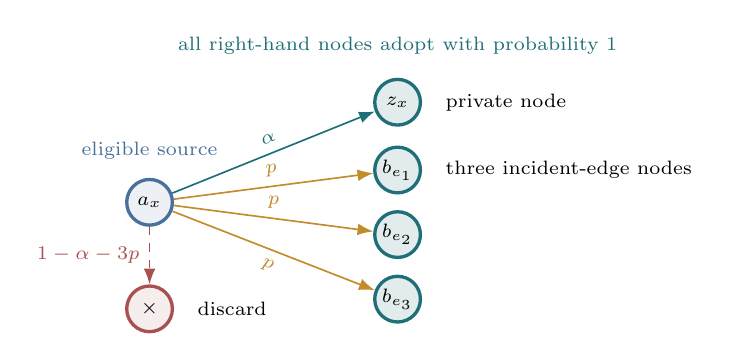
\begin{tikzpicture}[x=1cm,y=0.82cm]
    \node[cimseed] (ax) at (0,0) {$a_x$};
    \node[cimlabel,above=3pt of ax,text=cimBlue] {eligible source};
    \node[cimadopt] (zx) at (3.15,1.55) {$z_x$};
    \node[cimadopt] (b1) at (3.15,0.50) {$b_{e_1}$};
    \node[cimadopt] (b2) at (3.15,-0.50) {$b_{e_2}$};
    \node[cimadopt] (b3) at (3.15,-1.50) {$b_{e_3}$};
    \node[cimdrop] (drop) at (0,-1.65) {$\times$};

    \draw[cimarrow,cimTeal] (ax) -- node[above,sloped,cimlabel]
      {$\alpha$} (zx);
    \draw[cimarrow,cimGold] (ax) -- node[above,sloped,cimlabel]
      {$p$} (b1);
    \draw[cimarrow,cimGold] (ax) -- node[above,cimlabel]
      {$p$} (b2);
    \draw[cimarrow,cimGold] (ax) -- node[below,sloped,cimlabel]
      {$p$} (b3);
    \draw[cimarrow,cimRed,dashed] (ax) -- node[left,cimlabel]
      {$1-\alpha-3p$} (drop);

    \node[cimlabel,right=5pt of zx] {private node};
    \node[cimlabel,right=5pt of b1,anchor=west] {three incident-edge nodes};
    \node[cimlabel,right=5pt of drop] {discard};
    \node[cimlabel,above=5pt of zx,text=cimTeal]
      {all right-hand nodes adopt with probability $1$};
  \end{tikzpicture}
  \caption{The reduction gadget for a vertex $x$ in the cubic graph.
  Only $a_x$ is eligible for coupon allocation; a coupon reaches either
  the private node $z_x$, one of the three incident-edge nodes, or the
  discard outcome.}
  \Description{A source node has one edge to a private adopter, three
  edges to adopter nodes representing incident cubic-graph edges, and a
  dashed edge to a discard outcome.}
  \label{fig:hardness-gadget}
\end{figure}

We first show that an optimal allocation of $K$ coupons uses $K$
distinct sources, even though CIM permits repeated seeds.
Suppose an allocation places $r\geq2$ coupons at $a_x$ and none at $a_y$.
Removing one coupon from $a_x$ decreases the adoption probability of
$z_x$ by
$\alpha(1-\alpha)^{r-1}\leq\alpha(1-\alpha)$ and decreases the total
contribution of the three incident edge nodes by at most $3p$.
Placing that coupon at $a_y$ increases the adoption probability of its
previously uncovered private node $z_y$ by $\alpha$; any gain at edge
nodes is additional.
The net change is therefore at least
\[
  \alpha-\alpha(1-\alpha)-3p=\alpha^2-3p>0.
\]
Hence a repeated source cannot occur in an optimal allocation.

Consider now a set $S$ of $K$ distinct sources, and let
$c_e(S)\in\{0,1,2\}$ be the number of selected endpoints of edge $e$.
The private nodes contribute exactly $K\alpha$, while $b_e$ adopts with
probability $1-(1-p)^{c_e(S)}$.
Let $n_i$ be the number of edges with $c_e(S)=i$.
Since $H$ is cubic,
\[
  n_0+n_1+n_2=|E_H|,
  \qquad n_1+2n_2=3K.
\]
The total expected adoption spread is
\begin{align*}
  \sigma(S)
  &=K\alpha+n_1p+n_2(2p-p^2)\\
  &=K\alpha+3Kp-(3K-|E_H|)p^2-n_0p^2.
\end{align*}
It reaches
\[
  B=K\alpha+3Kp-(3K-|E_H|)p^2
\]
if and only if $n_0=0$, which holds exactly when the corresponding
vertices form a size-$K$ vertex cover of $H$.
Because an optimal allocation uses distinct sources, $H$ has a size-$K$
vertex cover if and only if the constructed CIM instance admits an allocation
with spread at least $B$. The construction is polynomial, so CIM is NP-hard.
\end{proof}

\subsection{Monotonicity and Submodularity}

Because several coupons may be assigned to the same seed, the natural
domain of CIM is the integer lattice $\mathbb{Z}_{\geq0}^{V_s}$.
For allocations $\bm{x}\leq\bm{y}$ componentwise and a candidate seed
$v$, let $\bm{e}_v$ denote one additional coupon at $v$.
A function $f$ has the diminishing-returns (DR) property if
\[
  f(\bm{x}+\bm{e}_v)-f(\bm{x})
  \geq
  f(\bm{y}+\bm{e}_v)-f(\bm{y}).
\]
This is the integer-lattice analogue of set-function submodularity.

\begin{theorem}
\label{thm:monosub}
For every coupon influence instance, $\sigma(\bm{x})$ is monotone and
DR-submodular over coupon allocations.
\end{theorem}

\begin{proof}
The marginal gain of assigning one additional coupon to $v$ is
\begin{align*}
  \Delta_v(\bm{x})
  &=\sigma(\bm{x}+\bm{e}_v)-\sigma(\bm{x})\\
  &=\sum_{u\in V}q_{vu}
    \prod_{w\in V_s}(1-q_{wu})^{x_w}.
\end{align*}
Every term is non-negative, so $\sigma$ is monotone.
If $\bm{x}\leq\bm{y}$, then for every user $u$,
\[
  \prod_{w\in V_s}(1-q_{wu})^{x_w}
  \geq
  \prod_{w\in V_s}(1-q_{wu})^{y_w}.
\]
Therefore $\Delta_v(\bm{x})\geq\Delta_v(\bm{y})$, proving the DR
property.
\end{proof}

Starting from $\bm{x}_0=\bm{0}$, exact greedy assigns coupon $i+1$ to
$v_i\in\arg\max_{v:x_{i,v}<c_v}\Delta_v(\bm{x}_i)$ for
$i=0,\ldots,k-1$.
Equivalently, we may replace each candidate $v$ by $c_v$ identical copies
and apply cardinality-constrained greedy to the resulting ground set.
The standard cardinality argument for monotone DR-submodular functions
gives
\[
  \sigma(\bm{x}_k)
  \geq \left(1-\left(1-\frac{1}{k}\right)^k\right)\sigma(\bm{x}^*)
  \geq (1-1/e)\sigma(\bm{x}^*)
\]
~\cite{nemhauser1978analysis}.

However, an exact greedy implementation is still inefficient, because
evaluating $\sigma(S)$ exactly is computationally expensive.
One may first estimate the full matrix $Q=(q_{vu})$ using many independent
single-coupon trajectories from every candidate seed and then evaluate all
greedy marginals, but this requires $O(n^2)$ storage and a large number of
forward simulations before seed selection begins.
One may also estimate $\sigma(S)$ by Monte Carlo simulation, but a
greedy algorithm would require repeated simulations for many candidate
seeds and many rounds, leading to a cost of
$O(k^2 |V_s|R\bar{L})$, where $R$ is the number of simulations and
$\bar{L}$ is the expected coupon-walk length.
Therefore, to make the monotone DR-submodular structure algorithmically
useful, we need an efficient estimator of the adoption spread.
In the next section, we develop such an estimator using $k$-joint
reverse reachable sets, and then build the \CIMRIS{} algorithm on top of
this estimator.

%% ============================================================
%% 5. ALGORITHM: CIM-RIS
%% ============================================================
\section{Algorithm: \CIMRIS{}}
\label{sec:algo}

We now design an efficient algorithm for CIM based on reverse
influence sampling.
We first define reverse reachable sets for single-coupon diffusion and
show their coverage property.
We then extend this construction to $k$ coupons by introducing
$k$-joint RR sets, which correctly preserve the coupling between the
$j$-th seed and the $j$-th coupon realization.
Finally, we use these samples to estimate the marginal gain of each
successive coupon and obtain the \CIMRIS{} algorithm.

\subsection{Reverse Reachable Sets for Coupon Diffusion}

The key insight of classical RIS is that influence maximization can be
turned into a maximum coverage problem over sampled \emph{reverse
reachable (RR) sets}.
In this section, we adapt this construction to the coupon influence
model.
The main difference is that a node becomes an adopter only when two events
occur simultaneously: the coupon reaches the node through a live-edge path,
and the node takes the adoption action in the corresponding realization.

\begin{definition}[Live edge]
Edge $(w,u) \in E$ is a \emph{live edge} in realization $W_j$ if\/
$\Phi_j(w)=u$.
\end{definition}

\paragraph{Single-coupon RR set.}
Fix a coupon index $j$ and its realization $W_j$.
For a target node $u$, we define the reverse reachable set
$R_j(u,W_j)$ as the set of seed nodes from which coupon $j$ reaches node $u$
and is redeemed there in this realization.
Formally,
\[
  R_j(u, W_j) =
  \begin{cases}
    \{w \in V : w \xrightarrow{*} u \text{ in } W_j\},
      & \text{if } A_{u,j} = 1, \\
    \emptyset, & \text{otherwise,}
  \end{cases}
\]
where $w\xrightarrow{*}u$ denotes a live-edge path from $w$ to $u$.
The condition $A_{u,j}=1$ is the adoption gate at the root node $u$.
If this gate does not fire, then no seed can cause $u$ to redeem coupon $j$
in realization $W_j$, and the reverse reachable set is empty.
If it does fire, then $R_j(u,W_j)$ contains exactly the nodes that can
reach $u$ through live edges in $W_j$.

\begin{lemma}[Coverage lemma]
\label{lem:coverage}
Coupon $j$ seeded at $s$ is redeemed by node $u$ in realization $W_j$ if
and only if $s \in R_j(u, W_j)$.
\end{lemma}

\begin{proof}
$\mathrm{Adopt}_{u,j}(s)$ requires (i) $A_{u,j} = 1$ and (ii) a
live-edge path from $s$ to $u$ in $W_j$.
Condition (i) is the adoption gate in the definition of $R_j(u,W_j)$,
and condition (ii) is precisely $s \in R_j(u, W_j)$.
\end{proof}

Lemma~\ref{lem:coverage} is the single-coupon analogue of the standard
RR-set coverage property: testing whether $s$ belongs to
$R_j(u,W_j)$ is equivalent to testing whether coupon $j$ seeded at $s$ is
redeemed by target node $u$ in realization $W_j$.

\paragraph{Why a naive union fails for $k$ coupons.}
For $k$ coupons assigned according to an ordered seed tuple
$(s_1,\ldots,s_k)$ under independent realizations
$(W_1,\ldots,W_k)$, node $v$ becomes an adopter if and only if
$\bigvee_{j=1}^k \{s_j \in R_j(v, W_j)\}$.
A tempting approach is to generate the union
$Q(v)=\bigcup_{j=1}^k R_j(v,W_j)$ and check whether any selected seed
falls in $Q(v)$.
This approach is incorrect because it ignores coupon identities.
If $s_i\in R_j(v,W_j)$ for some $i\neq j$, the union test would allow
seed $s_i$ to borrow the realization of coupon $j$, although coupon
$i$ and coupon $j$ propagate independently.
Therefore, correctness requires a per-coupon test: seed $s_j$ must be
checked only against $R_j(v,W_j)$.

\paragraph{$k$-joint RR sets.}
Based on the above observation, we define a \emph{$k$-joint RR set}
rooted at $v$ as the tuple
\[
  \mathcal{R}(v)=(R_1(v,W_1),\ldots,R_k(v,W_k)),
\]
where $W_1,\ldots,W_k$ are sampled independently.
The tuple keeps the correspondence between coupon index $j$ and its
own reverse reachable set $R_j(v,W_j)$.
For an ordered seed tuple $S=(s_1,\ldots,s_k)$, the sample is covered if
\[
  \bigvee_{j=1}^k \{s_j\in R_j(v,W_j)\}
\]
holds.
Figure~\ref{fig:joint-rr} illustrates why this index correspondence is
part of the sample rather than a bookkeeping detail.
This is the basic estimator used by \CIMRIS{}.

\begin{figure*}[t]
  \centering
  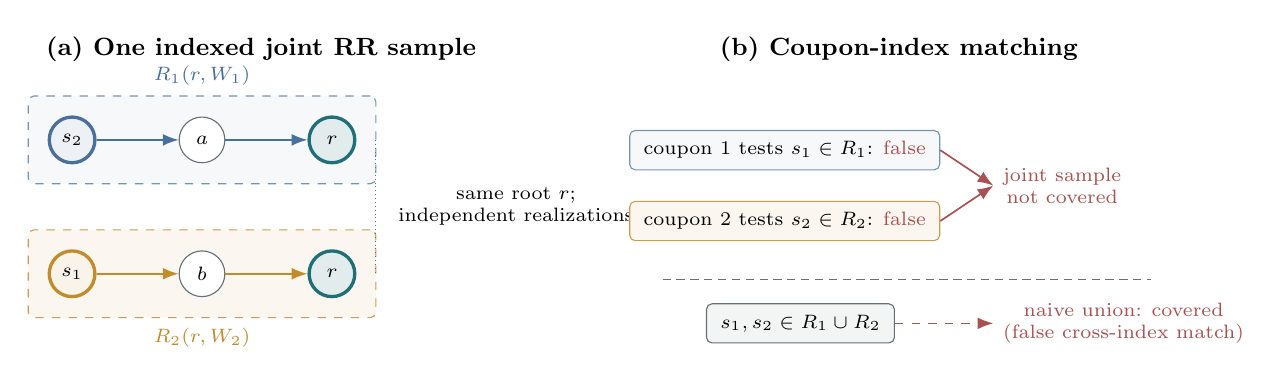
\begin{tikzpicture}[x=1cm,y=1cm]
    \begin{scope}
      \node[cimlabel,font=\small\bfseries] at (3.1,2.0)
        {(a) One indexed joint RR sample};
      \node[cimseed] (s2r1) at (0.7,0.85) {$s_2$};
      \node[cimnode] (a1) at (2.35,0.85) {$a$};
      \node[cimadopt] (r1) at (4.0,0.85) {$r$};
      \draw[cimarrow,cimBlue] (s2r1) -- (a1);
      \draw[cimarrow,cimBlue] (a1) -- (r1);

      \node[cimseed,draw=cimGold,fill=cimGold!10] (s1r2)
        at (0.7,-0.85) {$s_1$};
      \node[cimnode] (a2) at (2.35,-0.85) {$b$};
      \node[cimadopt] (r2) at (4.0,-0.85) {$r$};
      \draw[cimarrow,cimGold] (s1r2) -- (a2);
      \draw[cimarrow,cimGold] (a2) -- (r2);

      \begin{scope}[on background layer]
        \node[cimset,draw=cimBlue!75,fill=cimBlue!5,dashed,
              fit=(s2r1)(a1)(r1),inner sep=7pt,
              label={[cimlabel,text=cimBlue]above:$R_1(r,W_1)$}] {};
        \node[cimset,draw=cimGold!85,fill=cimGold!7,dashed,
              fit=(s1r2)(a2)(r2),inner sep=7pt,
              label={[cimlabel,text=cimGold]below:$R_2(r,W_2)$}] {};
      \end{scope}
      \draw[densely dotted,cimGray] (4.55,0.85) -- (4.55,-0.85);
      \node[cimlabel,anchor=west] at (4.72,0)
        {same root $r$;\\independent realizations};
    \end{scope}

    \begin{scope}[xshift=8.2cm]
      \node[cimlabel,font=\small\bfseries] at (3.0,2.0)
        {(b) Coupon-index matching};
      \node[cimset,draw=cimBlue!75,fill=cimBlue!5] (test1)
        at (1.55,0.72) {coupon 1 tests $s_1\in R_1$: \textcolor{cimRed}{false}};
      \node[cimset,draw=cimGold!85,fill=cimGold!7] (test2)
        at (1.55,-0.18) {coupon 2 tests $s_2\in R_2$: \textcolor{cimRed}{false}};
      \node[cimlabel,text=cimRed,anchor=west] (correct) at (4.2,0.27)
        {joint sample\\not covered};
      \draw[cimarrow,cimRed] (test1.east) -- (correct.west);
      \draw[cimarrow,cimRed] (test2.east) -- (correct.west);

      \draw[densely dashed,cimGray] (0,-0.92) -- (6.2,-0.92);
      \node[cimset,draw=cimGray,fill=cimLight] (union)
        at (1.75,-1.48) {$s_1,s_2\in R_1\cup R_2$};
      \node[cimlabel,text=cimRed,anchor=west] (wrong) at (4.2,-1.48)
        {naive union: covered\\(false cross-index match)};
      \draw[cimarrow,cimRed,dashed] (union.east) -- (wrong.west);
    \end{scope}
  \end{tikzpicture}
  \caption{A $k$-joint RR sample preserves the correspondence between
  coupon index $j$ and realization $W_j$ (shown for $k=2$).
  Coverage must test $s_j\in R_j$ with matching indices; taking the
  union of the RR sets can create a false cross-index match.}
  \Description{Two indexed reverse-reachable components share a root.
  Crossed seed memberships fail the index-matched coverage test but would
  be incorrectly accepted by an unindexed union.}
  \label{fig:joint-rr}
\end{figure*}

\begin{lemma}[Unbiasedness]
\label{lem:unbiased}
Let $v$ be drawn uniformly from $V$, and let
$(R_1(v, W_1), \ldots, R_k(v, W_k))$ be generated from $k$ independent
realizations rooted at $v$.
For any ordered seed tuple $S=(s_1,\ldots,s_k)$, we have
\[
  \sigma(S)
  = n\cdot
  \E\!\left[
    \I\!\left[\bigvee_{j=1}^{k} \{s_j \in R_j(v,W_j)\}\right]
  \right],
\]
or equivalently,
\[
  \E\!\left[
    \I\!\left[\bigvee_{j=1}^{k} \{s_j \in R_j(v,W_j)\}\right]
  \right]
  \;=\; \frac{\sigma(S)}{n}.
\]
\end{lemma}

\begin{proof}
The expectation is over the uniformly sampled root $v$ and over the
independent realizations $W_1,\ldots,W_k$.
\begin{align*}
  \E\!\left[
    \I\!\left[\bigvee_{j=1}^k \{s_j \in R_j(v,W_j)\}\right]
  \right]
  &= \frac{1}{n}\sum_{u\in V}
     \Pr\!\left[\bigvee_{j=1}^k \{s_j \in R_j(u,W_j)\}\right] \\
  &\stackrel{(*)}{=}
     \frac{1}{n}\sum_{u\in V}
     \Pr\!\left[\bigvee_{j=1}^k \mathrm{Adopt}_{u,j}(s_j)\right] \\
  &= \frac{\sigma(S)}{n},
\end{align*}
where step $(*)$ applies Lemma~\ref{lem:coverage} to each coupon realization.
The last equality follows from the definition of adoption spread.
\end{proof}

\subsection{Sampling Procedure}

The uniform-root construction in Lemma~\ref{lem:unbiased} is conceptually
simple, but it generates an empty joint sample whenever none of the root
adoption gates fires.
We avoid these zero-contribution samples by conditioning on the event that
at least one root-adoption gate fires.
For a root $v$, define
\[
  C_v=\bigvee_{j=1}^k A_{v,j},\qquad
  w_v=\Pr[C_v]=1-(1-p_v^a)^k,\qquad
  W=\sum_{v\in V}w_v.
\]
If $W=0$, no node can become an adopter and the optimal spread is zero, so we
assume $W>0$.
One conditioned joint sample is generated by (a) drawing root $v$ with
probability $w_v/W$; (b) drawing the vector of $k$ Bernoulli adoption
gates from its product distribution conditioned on $C_v$; and (c) for
every index $j$ whose gate fires,
generating $R_j(v,W_j)$ by a backward traversal over live in-edges.
The conditioned gate vector can be drawn in $O(k)$ time by sampling its
first firing index from the corresponding truncated geometric distribution
and then sampling all later gates independently.
Algorithm~\ref{alg:kernel} gives the deterministic transition kernel
for one node once the random number $r_{u,j}$ has been fixed.
This kernel is used lazily during the backward traversal so that the
same node-coupon pair has a consistent action within the same
realization.
The categorical action distribution of each node can be stored in an alias
table using $O(m+n)$ total preprocessing, allowing each action to be generated
and cached in $O(1)$ time while preserving the same distribution.

\begin{algorithm}[t]
\caption{Single-Node Transition Kernel}
\label{alg:kernel}
\begin{algorithmic}[1]
\Require Node $u$; coupon index $j$; random number $r_{u,j}$
\Require Parameters $p_u^a$, $p_u^d$,
  $\{p(u,v)\}_{v:(u,v)\in E}$
\Ensure Action
  $\Phi_j(u)\in\{\mathtt{adopt},\mathtt{discard}\}\cup N^+(u)$
\If{$r_{u,j} \leq p_u^a$}
  \State \Return $\mathtt{adopt}$
\ElsIf{$r_{u,j} \leq p_u^a + p_u^d$}
  \State \Return $\mathtt{discard}$
\Else
  \State Find $v^*$ such that $r_{u,j}$ falls in $v^*$'s transfer interval
  \State \Return $v^*$
\EndIf
\end{algorithmic}
\end{algorithm}

Algorithm~\ref{alg:rrset} implements the conditioned procedure.
For each coupon index $j$ with $A_{v,j}=1$, it performs a backward BFS.
When the traversal examines an in-neighbor $w$ of the current node, it
generates $r_{w,j}$ only if this random number has not been generated
before, and then checks whether $(w,u)$ is the live edge selected by
$w$ in realization $W_j$.
If so, $w$ is added to $R_j$; otherwise, this in-neighbor is ignored.

\begin{algorithm}[t]
\caption{Conditioned $k$-Joint RR Sample Generation}
\label{alg:rrset}
\begin{algorithmic}[1]
\Require Graph $G=(V,E)$; parameters $\{p_u^a, p_u^d, p(u,v)\}$;
  coupon count $k$; root weights $\{w_v\}$ and $W$
\Ensure $k$-joint RR sample $((R_1,\ldots,R_k),\; v)$
\State Sample root $v$ with probability $w_v/W$
\State Sample $(A_{v,1},\ldots,A_{v,k})$ from their product
  $\mathrm{Bernoulli}(p_v^a)$ distribution conditioned on $C_v$
\State $R_1, \ldots, R_k \gets \emptyset$
\For{$j = 1$ to $k$}
  \If{$A_{v,j} = 1$}
    \State $R_j \gets \{v\}$;\ \ $\text{queue} \gets [v]$
    \While{$\text{queue} \neq \emptyset$}
      \State $u \gets \text{queue.dequeue()}$
      \For{each in-neighbor $w$ of $u$}
        \If{$w \notin R_j$}
          \If{$r_{w,j}$ not yet sampled}
            \State $r_{w,j} \sim \mathrm{Uniform}[0,1]$
          \EndIf
          \If{$\Phi_j(w)=u$}
            \State $R_j \gets R_j \cup \{w\}$;\ \
              $\text{queue.enqueue}(w)$
          \EndIf
        \EndIf
      \EndFor
    \EndWhile
  \EndIf
\EndFor
\State \Return $((R_1, \ldots, R_k),\; v)$
\end{algorithmic}
\end{algorithm}

\begin{lemma}[Conditioned-root estimator]
\label{lem:importance}
Let $\mathcal{R}$ be generated by Algorithm~\ref{alg:rrset}, and let
\[
  Y(S_i)=\I\!\left[\bigvee_{j=1}^i\{s_j\in R_j\}\right]
\]
for any prefix $S_i=(s_1,\ldots,s_i)$ with $i\leq k$.
Then
\[
  \E[W Y(S_i)]=\sigma(S_i),
\]
where $\sigma(S_i)$ is the spread produced by the $i$ coupons in the
prefix.
\end{lemma}

\begin{proof}
For a fixed root $v$ with $w_v>0$, let $Y_v(S_i)$ be the coverage event
under the unconditioned realizations.
Coverage by any prefix implies that at least one of the first $i$ root
adoption gates fires. It therefore also implies the conditioning event over
all $k$ gates, so
$Y_v(S_i)\subseteq C_v$ and
$\Pr[Y_v(S_i)\mid C_v]=\Pr[Y_v(S_i)]/w_v$.
Taking expectation over the importance-sampled root gives
\begin{align*}
  \E[W Y(S_i)]
  &=\sum_{v\in V}\frac{w_v}{W}\,W\,
    \Pr[Y_v(S_i)\mid C_v]\\
  &=\sum_{v\in V}\Pr[Y_v(S_i)]
   =\sigma(S_i),
\end{align*}
where the final equality follows from Lemma~\ref{lem:coverage} and the
definition of adoption spread.
\end{proof}

\subsection{The \CIMRIS{} Algorithm}

Let $\mathcal{F}$ be a collection of $T$ independently generated
$k$-joint RR samples,
\[
  \mathcal{F} =
  \{((R_1^{(t)},\ldots,R_k^{(t)}),\,v^{(t)})\}_{t=1}^T.
\]
For a prefix $S_i=(s_1,\ldots,s_i)$ and sample $t$, define
\[
  Y_t(S_i)=
  \I\!\left[\bigvee_{j=1}^{i}\{s_j\in R_j^{(t)}\}\right].
\]
By Lemma~\ref{lem:importance},
$\hat{\sigma}(S_i)=W\sum_tY_t(S_i)/T$ is an unbiased spread estimator.
At round $i$, assigning coupon $i$ to $u$ newly covers sample $t$ exactly
when $Y_t(S_{i-1})=0$ and $u\in R_i^{(t)}$.
We therefore estimate its marginal gain by
\[
  \widehat{\Delta}_i(u\mid S_{i-1})
  =\frac{W}{T}\sum_{t=1}^{T}
    \I[Y_t(S_{i-1})=0]\,\I[u\in R_i^{(t)}].
\]

\begin{lemma}[Marginal-gain estimator]
\label{lem:marginal}
For every fixed prefix $S_{i-1}$ and feasible candidate
$u\in V_s$ with $x_u(S_{i-1})<c_u$,
\[
  \E[\widehat{\Delta}_i(u\mid S_{i-1})]
  =\sigma(\bm{x}(S_{i-1})+\bm{e}_u)
   -\sigma(\bm{x}(S_{i-1})).
\]
\end{lemma}

\begin{proof}
For a fixed root $v$, the first indicator means that none of the first
$i-1$ coupons is redeemed at $v$, while the second means that coupon $i$
seeded at $u$ is redeemed there.
Their conjunction is exactly the event that the additional coupon makes
$v$ a new adopter. This event implies the conditioning event $C_v$ even
though $C_v$ is defined using all $k$ coupon gates.
The same importance-reweighting calculation as in
Lemma~\ref{lem:importance} therefore gives
\[
  \E\!\left[W\I[Y_t(S_{i-1})=0]\I[u\in R_i^{(t)}]\right]
  =\sum_{v\in V}\Pr[v\text{ is newly adopted}].
\]
The sum on the right is the stated marginal gain.
\end{proof}

Let $N=|V_s|$, let $\mathrm{OPT}=\sigma(\bm{x}^*)$, and let
$\epsilon,\delta\in(0,1)$ and
$\mathrm{LB}\in(0,\mathrm{OPT}]$ be a valid lower bound.
We set
\[
  T=\left\lceil
    \frac{16k^2W}{\epsilon^2\mathrm{LB}^2}
    \left(k\ln N+\ln\frac{2k}{\delta}\right)
  \right\rceil.
\]
A deterministic choice is
\[
  \mathrm{LB}_{\mathrm{path}}
  =\max_{\substack{s=v_0\in V_s,\,v_\ell\in V\\
                   (v_0,\ldots,v_\ell)\text{ simple}}}
    p_{v_\ell}^a\prod_{h=0}^{\ell-1}p(v_h,v_{h+1}),
\]
the largest probability of following one seed-to-adopter path.
If this value is zero, then $\mathrm{OPT}=0$; otherwise it is a positive
lower bound on $\mathrm{OPT}$.
Because all path factors lie in $[0,1]$, a maximizing positive path can be
chosen simple; the value can be computed using shortest paths after applying
negative logarithms to positive transfer and adoption probabilities.
Independent pilot RR samples can give a tighter lower confidence bound in
practice.
The value of $T$ above is a sufficient theorem-level sample count: when
$\epsilon$, $\delta$, and a valid $\mathrm{LB}$ are supplied, it is the
quantity used to attach the high-probability guarantee in
Theorem~\ref{thm:approx} to one run.
Because the bound is uniform over all possible greedy prefixes, it can be
conservative in practice, particularly when $\mathrm{LB}$ is small.
An implementation may instead use a fixed empirical sample budget, but such a
run should be interpreted as an approximate RIS implementation without a
per-run $(\epsilon,\delta)$ certificate unless its budget also satisfies this
bound.
With these samples, \CIMRIS{} processes coupon indices in order and
selects the candidate with the largest empirical marginal gain.
Using inverted lists from node--coupon pairs to samples, the gains in
each round are computed by scanning RR memberships rather than all
candidate--sample pairs.

\begin{algorithm}[t]
\caption{\CIMRIS{}$(G,V_s,\bm{c},k,\epsilon,\delta,\mathrm{LB})$}
\label{alg:cim-ris}
\begin{algorithmic}[1]
\State Compute $w_v\gets1-(1-p_v^a)^k$ for all $v$ and
  $W\gets\sum_v w_v$
\If{$W=0$}
  \State \Return any feasible allocation with spread $0$
\EndIf
\State Set $T$ according to the sample-size equation above
\State Generate $T$ independent conditioned samples $\mathcal{F}$
  using Algorithm~\ref{alg:rrset}
\State $S_0\gets()$;\ $\bm{x}\gets\bm{0}$;\
  $\mathrm{covered}[t]\gets\mathrm{false}$ for every $t$
\For{$i=1$ to $k$}
  \For{$u\in V_s$ with $x_u<c_u$}
    \State $g(u)\gets
      |\{t:\neg\mathrm{covered}[t]\ \wedge\ u\in R_i^{(t)}\}|$
  \EndFor
  \State $s_i\gets\arg\max_{u\in V_s:x_u<c_u}g(u)$;\
    $\bm{x}\gets\bm{x}+\bm{e}_{s_i}$
  \For{each $t$ with $\neg\mathrm{covered}[t]$ and $s_i\in R_i^{(t)}$}
    \State $\mathrm{covered}[t]\gets\mathrm{true}$
  \EndFor
  \State $S_i\gets(S_{i-1},s_i)$
\EndFor
\State \Return allocation $\bm{x}$ and ordered tuple $S_k$
\end{algorithmic}
\end{algorithm}

\subsection{Theoretical Guarantees}

\begin{theorem}
\label{thm:approx}
Let $\mathrm{LB}\in(0,\mathrm{OPT}]$ and let $T$ be chosen as above.
\CIMRIS{} returns an allocation $\hat{\bm{x}}$ satisfying, with
probability at least $1-\delta$,
\[
  \sigma(\hat{\bm{x}})
  \geq (1-1/e-\epsilon)\,\mathrm{OPT}.
\]
Its expected running time is
\[
  O\!\left(
    \frac{k^3(m+n)}{\epsilon^2\mathrm{LB}^2}
    \left(k\ln |V_s|+\ln\frac{k}{\delta}\right)
    +k|V_s|
  \right).
\]
\end{theorem}

\begin{proof}
\textit{Approximation.}
Lemma~\ref{lem:marginal} shows that every coverage count used by the
algorithm is an unbiased estimate of the corresponding true marginal
gain.
There are at most
$\sum_{i=1}^k |V_s|^i\leq k|V_s|^k$ prefix--candidate combinations over
all possible executions.
For a fixed combination, define
\[
  Z_t=W\I[Y_t(S_{i-1})=0]\I[u\in R_i^{(t)}].
\]
Then $0\leq Z_t\leq W$, $\E[Z_t]=\Delta_u(\bm{x}(S_{i-1}))$,
and this marginal is at most one because one additional coupon can
create at most one new adopter.
Consequently,
$\operatorname{Var}(Z_t)\leq\E[Z_t^2]\leq W\E[Z_t]\leq W$.
Bernstein's inequality therefore gives
\[
  \Pr\!\left[
    |\widehat{\Delta}_i(u\mid S_{i-1})
      -\Delta_u(\bm{x}(S_{i-1}))|>\tau
  \right]
  \leq
  2\exp\!\left(
    -\frac{T\tau^2}{2W+(2/3)W\tau}
  \right).
\]
Set $\tau=\epsilon\mathrm{LB}/(2k)$.
Since $\mathrm{LB}\leq\mathrm{OPT}\leq k$, we have $\tau\leq1/2$.
Let $L=k\ln|V_s|+\ln(2k/\delta)$.
The denominator in the Bernstein exponent is at most $7W/3$, whereas
$T\tau^2\geq4WL$.
Thus the failure probability for one combination is at most
$2e^{-L}=\delta/(k|V_s|^k)$.
A union bound makes every marginal estimate accurate within $\tau$
simultaneously with probability at least $1-\delta$.
On this event, the candidate selected in each round has true marginal
gain at least the largest feasible marginal minus
$2\tau=\epsilon\mathrm{LB}/k$.

Let $\bm{x}_i$ be the allocation after round $i$, and let
$\bm{x}_i\vee\bm{x}^*$ denote the componentwise maximum of $\bm{x}_i$ and
an optimal allocation. Monotonicity and DR-submodularity give
\[
  \mathrm{OPT}-\sigma(\bm{x}_i)
  \leq \sigma(\bm{x}_i\vee\bm{x}^*)-\sigma(\bm{x}_i)
  \leq \sum_{v\in V_s}(x_v^*-x_{i,v})_+\Delta_v(\bm{x}_i).
\]
Every term with $(x_v^*-x_{i,v})_+>0$ is feasible because
$x_{i,v}<x_v^*\leq c_v$, and the coefficients sum to at most $k$.
Therefore,
\[
  \max_{v\in V_s:x_{i,v}<c_v}\Delta_v(\bm{x}_i)
  \geq \frac{\mathrm{OPT}-\sigma(\bm{x}_i)}{k}.
\]
Combining this inequality with the concentration event gives
\[
  \mathrm{OPT}-\sigma(\bm{x}_{i+1})
  \leq
  \left(1-\frac{1}{k}\right)
  \bigl(\mathrm{OPT}-\sigma(\bm{x}_i)\bigr)
  +
  \frac{\epsilon\mathrm{LB}}{k}.
\]
Writing $g_i=\mathrm{OPT}-\sigma(\bm{x}_i)$ and iterating this recurrence
for $k$ rounds yields
\begin{align*}
  g_k
  &\leq \left(1-\frac{1}{k}\right)^k\mathrm{OPT}
    +\frac{\epsilon\mathrm{LB}}{k}
      \sum_{r=0}^{k-1}\left(1-\frac{1}{k}\right)^r \\
  &\leq e^{-1}\mathrm{OPT}+\epsilon\mathrm{LB}
  \leq (e^{-1}+\epsilon)\mathrm{OPT}.
\end{align*}
Hence
$\sigma(\bm{x}_k)\geq(1-1/e-\epsilon)\mathrm{OPT}$.

\textit{Complexity.}
Let $q_{wv}$ be the probability that one coupon seeded at $w$ is redeemed
by $v$.
For coupon index $j$, the event $w\in R_j(v,W_j)$ implies $C_v$, and
hence, for every root with $w_v>0$,
\[
  \Pr[w\in R_j(v,W_j)\mid C_v]=\frac{q_{wv}}{w_v}.
\]
After averaging over the root distribution $w_v/W$, the expected total
number of node memberships in one conditioned joint sample is
\[
  \frac{k}{W}\sum_{w\in V}\sum_{v\in V}q_{wv}
  \leq\frac{kn}{W}.
\]
The inequality holds because a coupon seeded at $w$ can be redeemed by at
most one node, so $\sum_vq_{wv}\leq1$.
The corresponding expected number of scanned in-edges is
\[
  \frac{k}{W}\sum_{w\in V}d^-(w)\sum_{v\in V}q_{wv}
  \leq\frac{km}{W}.
\]
Sampling the conditioned root gates takes $O(k)$ time, which is absorbed
because $W\leq n$.
Alias tables for the root and node-action distributions take $O(m+n)$ total
preprocessing time; afterward, each root and each newly encountered node action
can be sampled in $O(1)$ time.
Thus one conditioned joint sample costs
$O(k(m+n)/W)$ in expectation.
Multiplying by $T$ cancels $W$ and gives the first term in the stated
bound.
The ceiling in $T$ and the $O(m+n)$ preprocessing do not change this order.
Indeed, $\mathrm{OPT}\leq k$ because each coupon creates at most one
adopter, and $\mathrm{OPT}\leq W$ because adoption at root $v$ implies
$C_v$; hence $\mathrm{LB}\leq\min\{k,W\}$.
These inequalities ensure that the stated sampling term also dominates the
cost of one additional sample from the ceiling and the preprocessing cost.
Finally, inverted RR-membership lists account for the sample-processing
work, while initializing candidate gains in each round costs
$O(k|V_s|)$.
\end{proof}

Compared with classical RIS, the additional dependence on $k$ is caused
by independent coupon realizations and sequential marginal estimation.
The explicit dependence on $\mathrm{LB}$ reflects the fact that adoption
probabilities can be arbitrarily small: unlike classical IM, a seed user is
not automatically counted as an adopter.

%% ============================================================
%% 6. EXPERIMENTS
%% ============================================================
\section{Experiments}
\label{sec:exp}

Our evaluation addresses four questions:
(Q1) how closely does \CIMRIS{} approach Monte Carlo greedy;
(Q2) how do broadcast-IM and structural baselines behave under coupon
diffusion; (Q3) when does conditioned root sampling improve estimator
efficiency; and (Q4) how does running time scale with the coupon budget
and graph size?
We use five graph instances derived from real networks and three parameter
regimes that balance adoption, discard, and forwarding differently.

\subsection{Experimental Setup}
\label{sec:exp-setup}

\paragraph{Datasets.}
We use five graph instances derived from real networks in the KONECT
collection~\cite{kunegis2013konect}, with basic statistics shown in
Table~\ref{tab:datasets}.
The Netscience dataset is a scientific collaboration network, EmailEnron
is an email communication network, and NetFacebookEgo and Douban are
online social networks. DoubanRandom is a sampled Douban instance.
We represent each undirected contact by two directed edges.
The four smaller graphs form the primary quality suite, while
network.douban is reserved for scalability tests.

\begin{table}[t]
  \caption{Datasets used in the experiments.}
  \label{tab:datasets}
  \centering
  \resizebox{\columnwidth}{!}{%
  \begin{tabular}{lrrrrr}
    \toprule
    Dataset         & $|V|$   & $|E|$     & Avg.\ deg. & Max outdeg. & Sparsity \\
    \midrule
    Netscience      & 379     & 1,828     & 4.82    & 34    & 98.72\% \\
    NetFacebookEgo  & 2,888   & 5,962     & 2.06    & 769   & 99.93\% \\
    DoubanRandom    & 4,723   & 11,774    & 2.49    & 45    & 99.95\% \\
    EmailEnron      & 33,696  & 361,622   & 10.73   & 1,383 & 99.97\% \\
    network.douban  & 154,907 & 654,206   & 4.22    & 287   & 99.97\% \\
    \bottomrule
  \end{tabular}}
\end{table}

\paragraph{Diffusion parameters.}
Node probabilities are generated by the degree-based log-continuous
procedure in Algorithm~\ref{alg:gendist}. This procedure creates
heterogeneous behavior in which high-degree hubs adopt less and discard more;
their transfer probabilities depend on the scenario parameters.
The normalized log-degree $\hat{d}_u$ controls how $p_u^a$ and $p_u^d$
scale with degree.

\begin{algorithm}[t]
\caption{Degree-Based Node Probability Generation}
\label{alg:gendist}
\begin{algorithmic}[1]
\Require Degrees $\{d_u\}$; parameters
  $(\mathit{base}_a, \mathit{slope}_a, \mathit{base}_d,
    \mathit{slope}_d, h)$
\Ensure $\{p_u^a, p_u^d, p_u^t\}$ for all $u$
\For{$u \in V$}
  \State $\hat{d}_u \gets
    \bigl[\min\{1,\max\{10^{-5},
    \log(1{+}d_u)/\max_w\log(1{+}d_w)\}\}\bigr]^h$
\EndFor
\For{$u \in V$}
  \State $p_u^a \gets \mathit{base}_a
    + \mathit{slope}_a \cdot (1-\hat{d}_u)$
    \Comment{Low-degree nodes adopt more}
  \State $p_u^d \gets \mathit{base}_d
    + \mathit{slope}_d \cdot \hat{d}_u$
    \Comment{High-degree nodes discard more}
  \State $p_u^t \gets 1 - p_u^a - p_u^d$
  \If{$d_u=0$}
    \State $p_u^d\gets p_u^d+p_u^t$;\quad $p_u^t\gets0$
  \EndIf
\EndFor
\State $p(u,v) \gets p_u^t / d_u$ for every node with $d_u>0$
\State \Return $\{(p_u^a, p_u^d, p_u^t)\}_{u\in V}$
\end{algorithmic}
\end{algorithm}

We evaluate three scenarios reflecting distinct real-world campaign
settings, as summarized in Table~\ref{tab:scenarios}:

\begin{table}[t]
  \caption{Parameter settings for the three diffusion scenarios.}
  \label{tab:scenarios}
  \centering
  \begin{tabular}{lcccc}
    \toprule
    Scenario & $\mathit{base}_a$ & $\mathit{slope}_a$ &
              $\mathit{base}_d$ & $\mathit{slope}_d$ \\
    \midrule
    I.\ Balanced       & 0.30 & 0.10 & 0.10 & 0.10 \\
    II.\ Adoption-heavy & 0.45 & 0.35 & 0.15 & 0.05 \\
    III.\ Forwarding-heavy & 0.01 & 0.05 & 0.01 & 0.05 \\
    \bottomrule
  \end{tabular}
\end{table}

\begin{itemize}[leftmargin=*]
  \item \textbf{Scenario I (Balanced):}
    A balanced campaign in which adoption and forwarding coexist at
    moderate rates; the parameterization gives $p_u^t=0.50$ for every
    node.
  \item \textbf{Scenario II (Adoption-heavy):}
    Adoption probabilities range from $0.45$ to $0.80$, making immediate
    redemption more important than in Scenario I.
  \item \textbf{Scenario III (Forwarding-heavy):}
    The parameterization gives $p_u^t=0.93$ for every node, so coupons
    trace substantially longer forwarding paths.
    Adoption is rare at each step, but coupons travel farther, making
    multi-hop graph structure more relevant.
\end{itemize}

These degree-conditioned probabilities are controlled stress-test
parameters rather than estimates from observed coupon campaigns.
Accordingly, the experiments establish behavior under the stated model
on real network topologies, not external validity for a particular
commercial deployment.

\paragraph{Baselines.}
\CIMRIS{} is compared against two groups of methods.

\noindent\textit{Coupon-aware and structural heuristics.}
\begin{itemize}[leftmargin=*]
  \item \textbf{MC-Greedy}: Estimates the single-coupon adoption
    probabilities $q_{vu}$ from independent forward trajectories and
    applies exact greedy to the resulting estimated objective.
    We use $100{,}000$ trajectories per source on Netscience and
    $50{,}000$ per source on NetFacebookEgo in every scenario.
    Reference construction and final forward evaluation use independent
    random streams. Because constructing the full estimated matrix is
    expensive, this quality reference is limited to these two graphs.
  \item \textbf{1Hop-Sort}: Ranks nodes by expected one-step adoption
    score $p_u^a + \sum_{v \in N^+(u)} p(u,v)\,p_v^a$ and selects
    top-$k$.
  \item \textbf{Alpha-Sort}: Selects top-$k$ nodes by $p_u^a$.
  \item \textbf{DegreeTopM}: Selects top-$k$ nodes by out-degree.
  \item \textbf{PageRank}: Selects top-$k$ nodes by PageRank
    score~\cite{page1999pagerank}.
  \item \textbf{Random}: $k$ seeds drawn uniformly at random;
    lower-bound reference.
\end{itemize}

\noindent\textit{IC-model adaptation (model-mismatch baseline).}
\begin{itemize}[leftmargin=*]
  \item \textbf{IC-RIS}: Generates standard RR sets under the IC model
    with edge probabilities $p(u,v)$ and applies greedy maximum coverage
    using the same sample budget as \CIMRIS{}.
    This baseline follows the core RIS construction used by scalable IM
    methods~\cite{borgs2014maximizing,tang2015influence} while isolating
    the effect of replacing single-path coupon diffusion with broadcast
    diffusion.
\end{itemize}

The IC baseline tests whether broadcast-oriented reverse sampling can
compensate for model mismatch.

\paragraph{Evaluation metrics.}
For the main comparison, we set $V_s=V$ and $c_v=1$ for all methods, matching
the conventional distinct-seed policy used by the IM baselines.
\CIMRIS{} uses the adoption-root importance sampler described in
Section~\ref{sec:algo}; no path-success surrogate is used.
Each seed allocation is evaluated by averaging two quantities over $10{,}000$
independent Monte Carlo simulations of the $k$-coupon influence process:
(a) \emph{adoption spread}: distinct users who redeem at least one coupon
(primary objective); and (b) \emph{total redemptions}: redeemed coupons,
including multiple redemptions by the same user (secondary metric).
We use $k\in\{10,25,50,100,150,200\}$.

\paragraph{Implementation and reproducibility.}
All methods are implemented in Python~3.8 and evaluated on a machine with
eight AMD EPYC 9654 cores and 16~GB of memory; the reported selection
times use one process. The NetFacebookEgo MC-Greedy matrix is generated
in 32 chunks using eight processes; this preprocessing time is not included
in method selection times. We use five independent selection seeds
($20260715$--$20260719$).
The joint-sample budget is fixed before the cross-method comparison:
$100{,}000$ samples for $k\leq50$ and $50{,}000$ samples for $k\geq100$.
IC-RIS uses the same sample budget as \CIMRIS{}.
This two-level schedule was fixed from a pre-comparison convergence pilot.
It limits total sampling work because one joint sample contains up to $k$ RR
components and therefore becomes more expensive as the coupon budget grows;
the change at $k=100$ is not an adaptive stopping decision based on the
reported method outcomes.
These fixed budgets support a controlled empirical comparison; they are
not presented as the generally conservative sample count in
Theorem~\ref{thm:approx} for a particular $(\epsilon,\delta)$ pair.
Every selected allocation is evaluated with $10{,}000$ fresh forward
realizations, and methods within one configuration use common random-number
streams.
Figure error bars for \CIMRIS{} show 95\% confidence intervals over the
five selection runs.
Across the 72 graph--scenario--budget configurations, the adoption spread
has a mean cross-seed coefficient of variation of $0.51\%$ and a maximum
of $3.07\%$; the mean relative range is $1.27\%$.

\begin{figure*}[!t]
  \centering
  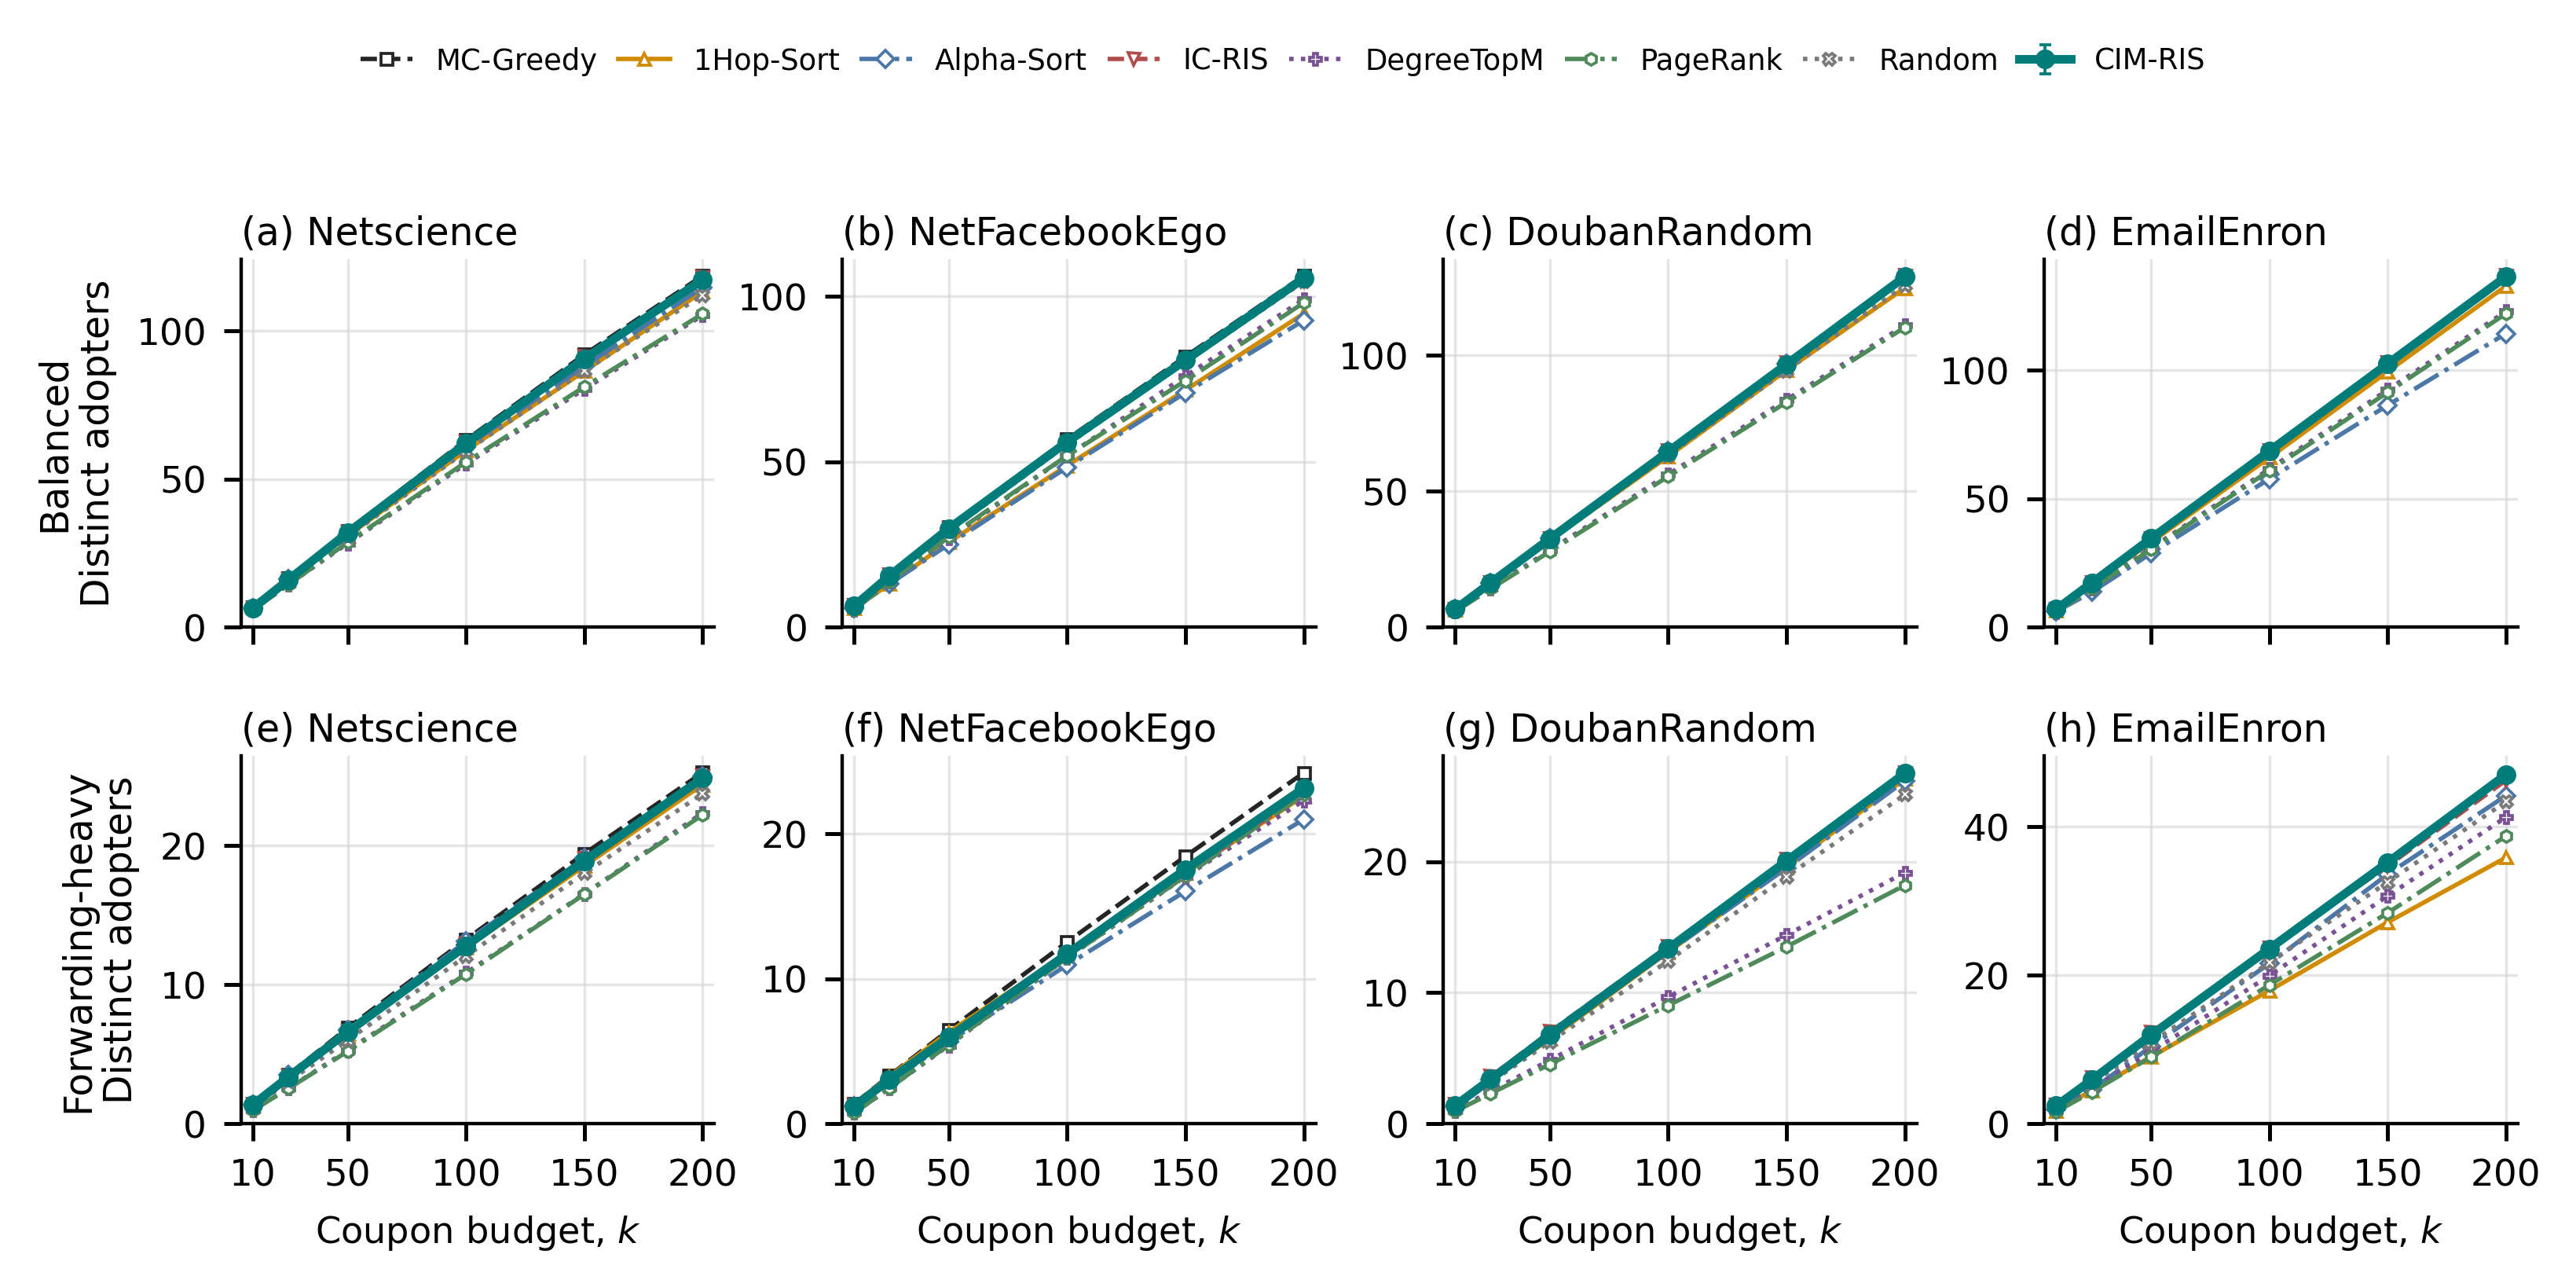
\includegraphics[width=0.87\textwidth]{figures/experiments/validated_quality_combined}
  \caption{Adoption spread in the balanced (top) and forwarding-heavy
  (bottom) scenarios. Each point is the mean of five selection runs, each
  evaluated using $10{,}000$ forward realizations; \CIMRIS{} error bars
  show 95\% confidence intervals across runs. MC-Greedy is reported on
  Netscience and NetFacebookEgo.}
  \Description{Eight line charts compare distinct adopters versus coupon
  budget across four networks and two diffusion scenarios.}
  \label{fig:real-quality}
\end{figure*}

\subsection{Solution Quality}
\label{sec:exp-quality}

Table~\ref{tab:aggregate-quality} summarizes the mean relative difference
between \CIMRIS{} and each baseline across the three scenarios. For each
graph--budget pair, the relative difference is
$100(\bar{\sigma}_{\mathrm{CIM\text{-}RIS}}-
\bar{\sigma}_{\mathrm{base}})/\bar{\sigma}_{\mathrm{base}}$.
It complements the budget-level results in
Figure~\ref{fig:real-quality} and reports
the adoption-heavy results without adding another four-panel figure.

\begin{table}[t]
  \caption{Mean relative adoption-spread difference (\%) between
  \CIMRIS{} and each baseline. Positive values favor \CIMRIS{}.
  Baseline comparisons average 24 graph--budget pairs per scenario;
  MC-Greedy averages the six Netscience budgets.}
  \label{tab:aggregate-quality}
  \centering
  \resizebox{\columnwidth}{!}{%
  \begin{tabular}{lrrrrr}
    \toprule
    Scenario & MC-Greedy & 1Hop-Sort & IC-RIS & DegreeTopM & PageRank \\
    \midrule
    Balanced         & $-2.3$ & $+5.8$ & $-0.1$ & $+12.6$ & $+13.3$ \\
    Adoption-heavy   & $-2.3$ & $-0.6$ & $+1.4$ & $ +9.5$ & $ +8.9$ \\
    Forwarding-heavy & $-3.4$ & $+8.5$ & $-0.7$ & $+25.5$ & $+30.2$ \\
    \bottomrule
  \end{tabular}}
\end{table}

The upper row of Figure~\ref{fig:real-quality} reports budget-level adoption
spread in the balanced scenario.
On Netscience, \CIMRIS{} is within $1.1$--$3.8\%$ of the MC-Greedy
reference over all six budgets, with a mean gap of $2.3\%$.
Across the four quality graphs, \CIMRIS{} outperforms 1Hop-Sort at 23 of
24 graph--budget pairs, with a mean relative improvement of $5.8\%$.
It also outperforms DegreeTopM and PageRank at every pair, by $12.6\%$
and $13.3\%$ on average, respectively.
IC-RIS is effectively tied in this scenario: each method wins 12 of the
24 graph--budget comparisons and the mean difference is $0.1\%$ in favor
of IC-RIS.
This result is consistent with the balanced parameters, under which
immediate adoption is common and local scores already provide useful
seed information.
The secondary redemption counts also confirm that the distinct-adopter
objective is not interchangeable with coupon utilization.
For example, at $k=200$ on NetFacebookEgo, \CIMRIS{} produces an average
of 128.8 redemptions but only 105.4 distinct adopters; duplicate
redemptions account for $18.1\%$ of the redeemed coupons.

The lower row of Figure~\ref{fig:real-quality} shows the forwarding-heavy
stress test.
Absolute spread is lower because per-visit adoption is rare.
The mean gap from MC-Greedy on Netscience is $3.4\%$ and decreases to
$1.5\%$ at $k=200$.
Across all graph--budget pairs, \CIMRIS{} outperforms 1Hop-Sort at 20 of
24 points and by $8.5\%$ on average.
Its mean improvements over DegreeTopM and PageRank increase to $25.5\%$
and $30.2\%$, respectively, and it wins all 24 comparisons against each.
IC-RIS remains competitive and is $0.7\%$ higher on average, showing that
model fidelity does not imply uniform empirical dominance at a fixed
sample budget.
The adoption-heavy scenario gives an intermediate pattern: the mean
Netscience gap to MC-Greedy is $2.3\%$, while \CIMRIS{} outperforms
IC-RIS at 23 of 24 points and by $1.4\%$ on average.
It again beats both topology-only rankings at all 24 points, although
1Hop-Sort is $0.6\%$ higher on average when immediate adoption dominates.

\begin{figure*}[t]
  \centering
  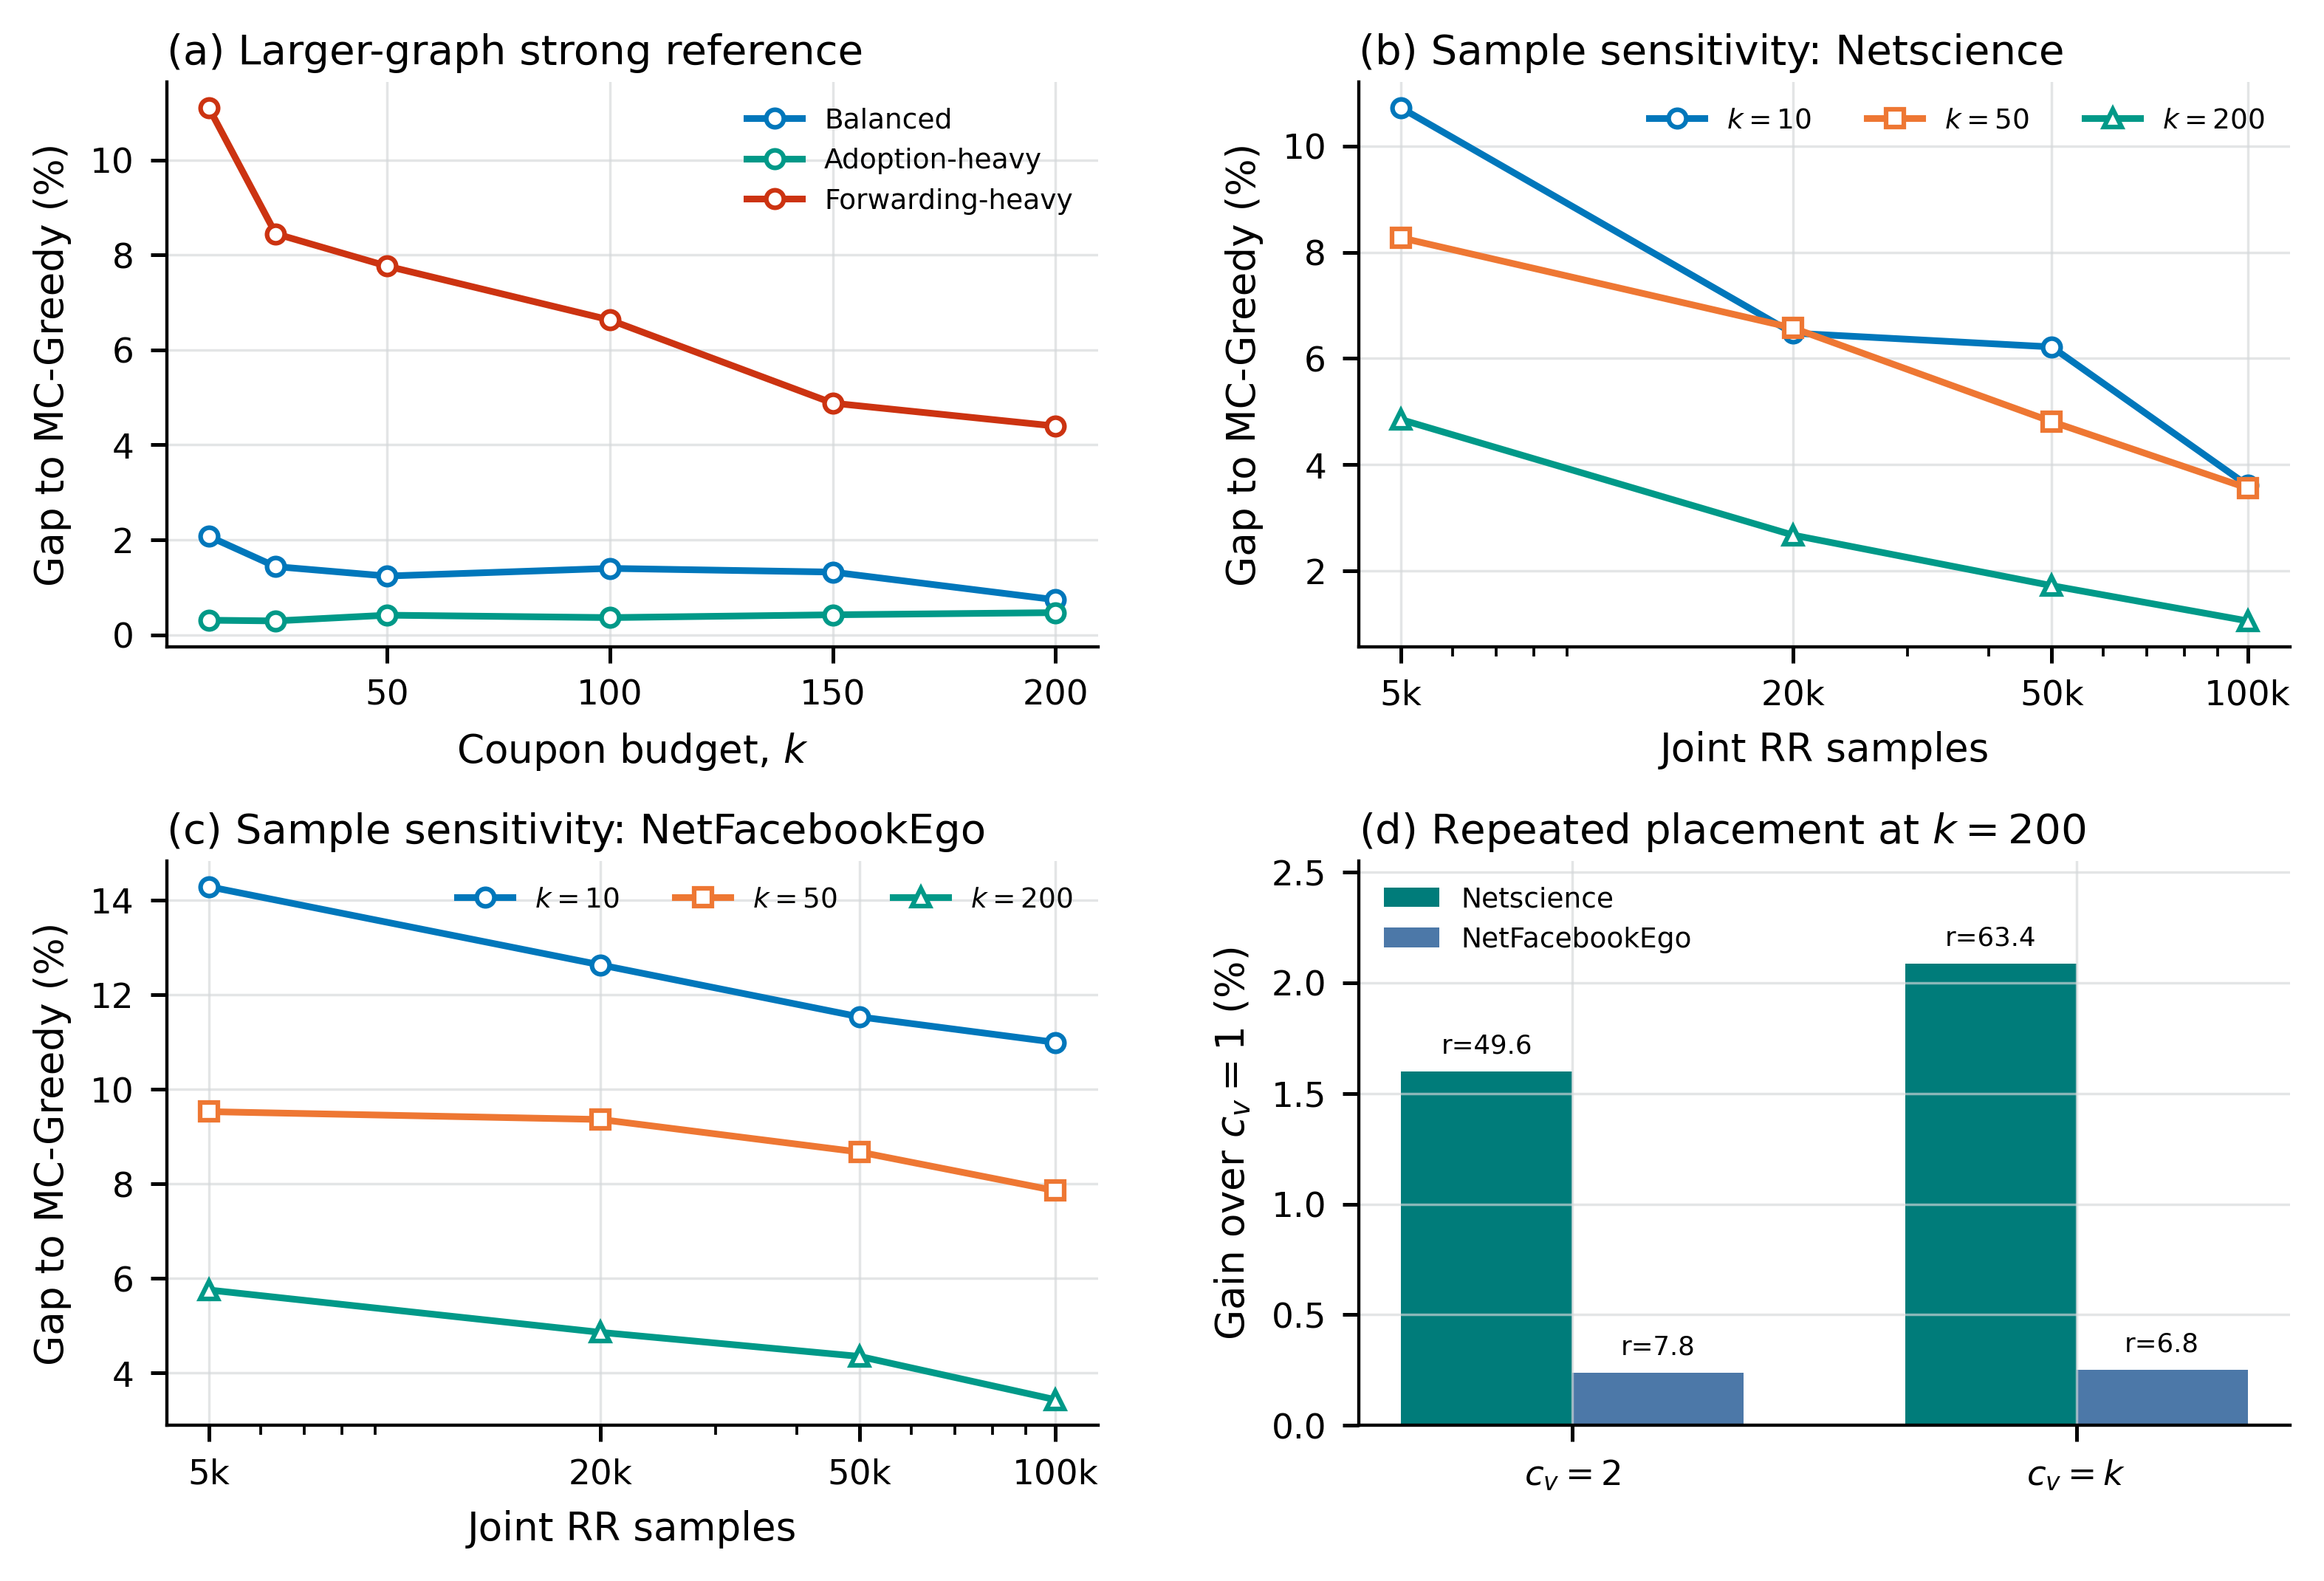
\includegraphics[width=0.91\textwidth]{figures/experiments/validated_extension_evidence}
  \caption{Strong-reference and robustness results. (a) Gap to
  MC-Greedy on NetFacebookEgo. (b--c) Effect of the joint RR sample count
  in the forwarding-heavy scenario. (d) Spread gain from relaxing the
  per-node capacity at $k=200$; labels report the mean number of repeated
  placements. Every reported statistic aggregates five \CIMRIS{} selection
  seeds, with $10{,}000$ forward realizations per evaluated allocation.}
  \Description{Four panels show the gap to Monte Carlo greedy on
  NetFacebookEgo, sample-count sensitivity on two networks, and the gain
  from allowing repeated coupon placement.}
  \label{fig:extension-evidence}
\end{figure*}

\subsection{Reference Strength, Sample Sensitivity, and Capacity}
\label{sec:exp-robustness}

We extend the strong-reference comparison from Netscience to
NetFacebookEgo using $50{,}000$ independent trajectories per source.
Figure~\ref{fig:extension-evidence}(a) shows that the mean gaps are
$1.37\%$ in the balanced scenario and $0.38\%$ in the adoption-heavy
scenario. The forwarding-heavy case is harder: the gap decreases from
$11.1\%$ at $k=10$ to $4.4\%$ at $k=200$, with a mean of $7.2\%$.
Across the two reference graphs, all three scenarios, and all six budgets,
the observed gap ranges from $0.3\%$ to $11.1\%$.
These results strengthen the comparison beyond the small Netscience graph,
but also identify low-budget, low-adoption diffusion as the least favorable
regime for the fixed empirical sample budget.

Figures~\ref{fig:extension-evidence}(b) and
\ref{fig:extension-evidence}(c) vary the number of joint RR samples in the
forwarding-heavy scenario while holding the evaluation streams fixed.
For every combination of the two graphs and $k\in\{10,50,200\}$, increasing
the sample count from $5{,}000$ to $100{,}000$ reduces the mean gap to
MC-Greedy. Averaged over the six combinations, the gap decreases from
$8.90\%$ to $5.09\%$. The improvement is largest on Netscience at
$k=10$, where the gap falls from $10.72\%$ to $3.61\%$, while
NetFacebookEgo at $k=10$ remains the hardest case, decreasing from
$14.29\%$ to $11.00\%$. Thus the sampling budget explains part, but not
all, of the remaining difference from MC-Greedy.
The corresponding running times expose the expected cost--accuracy trade-off.
Averaged over the six network--budget combinations, selection time grows from
$0.266$ seconds with $5{,}000$ samples to $1.016$, $2.435$, and $4.741$
seconds with $20{,}000$, $50{,}000$, and $100{,}000$ samples, respectively.
Over the same budgets, the mean gap decreases from $8.90\%$ to $7.10\%$,
$6.22\%$, and $5.09\%$.
Runtime is therefore approximately proportional to the number of samples,
whereas the observed quality improvement has diminishing returns.
This trade-off motivates the fixed two-level schedule in the main comparison,
but does not turn that empirical schedule into the theorem-calibrated value of
$T$.

Finally, Figure~\ref{fig:extension-evidence}(d) evaluates the capacity
formulation at $k=200$ under $c_v=1$, $c_v=2$, and $c_v=k$.
In the balanced and adoption-heavy scenarios, both \CIMRIS{} and
MC-Greedy almost always choose distinct seeds even when repetition is
allowed, so relaxing capacity has no material effect.
In the forwarding-heavy scenario, \CIMRIS{} uses an average of
$49.6$--$63.4$ repeated placements on Netscience and improves spread by
$1.60$--$2.09\%$ over $c_v=1$; on NetFacebookEgo, it uses
$6.8$--$7.8$ repeated placements and improves spread by about $0.25\%$.
Repeated placement is therefore useful when long trajectories make a
small group of sources repeatedly valuable, but it is not uniformly
beneficial across diffusion regimes.

\FloatBarrier

\subsection{Conditioned Sampling and Scalability}
\label{sec:exp-efficiency}

Figure~\ref{fig:real-sampler} isolates the conditioned-root sampler in
the forwarding-heavy scenario.
At $k=10$, uniform-root sampling spends $68.4\%$ of its Netscience
samples and $61.0\%$ of its EmailEnron samples on realizations in which
no root adoption gate fires.
Conditioning removes this work and reduces the coefficient of variation
from $0.128$ to $0.087$ on Netscience and from $0.809$ to $0.492$ on
EmailEnron.
After accounting for sampling time, the corresponding variance--time
improvements are $1.30\times$ and $1.53\times$.
Across all six measured conditions, the observed variance--time ratio is
between $1.30\times$ and $1.59\times$ in favor of conditioning.
By $k=200$, however, fewer than $0.3\%$ of uniform-root samples have no
firing gate, so differences in empirical variance should be interpreted
with the finite 30-batch sample size in mind.

\begin{figure}[t]
  \centering
  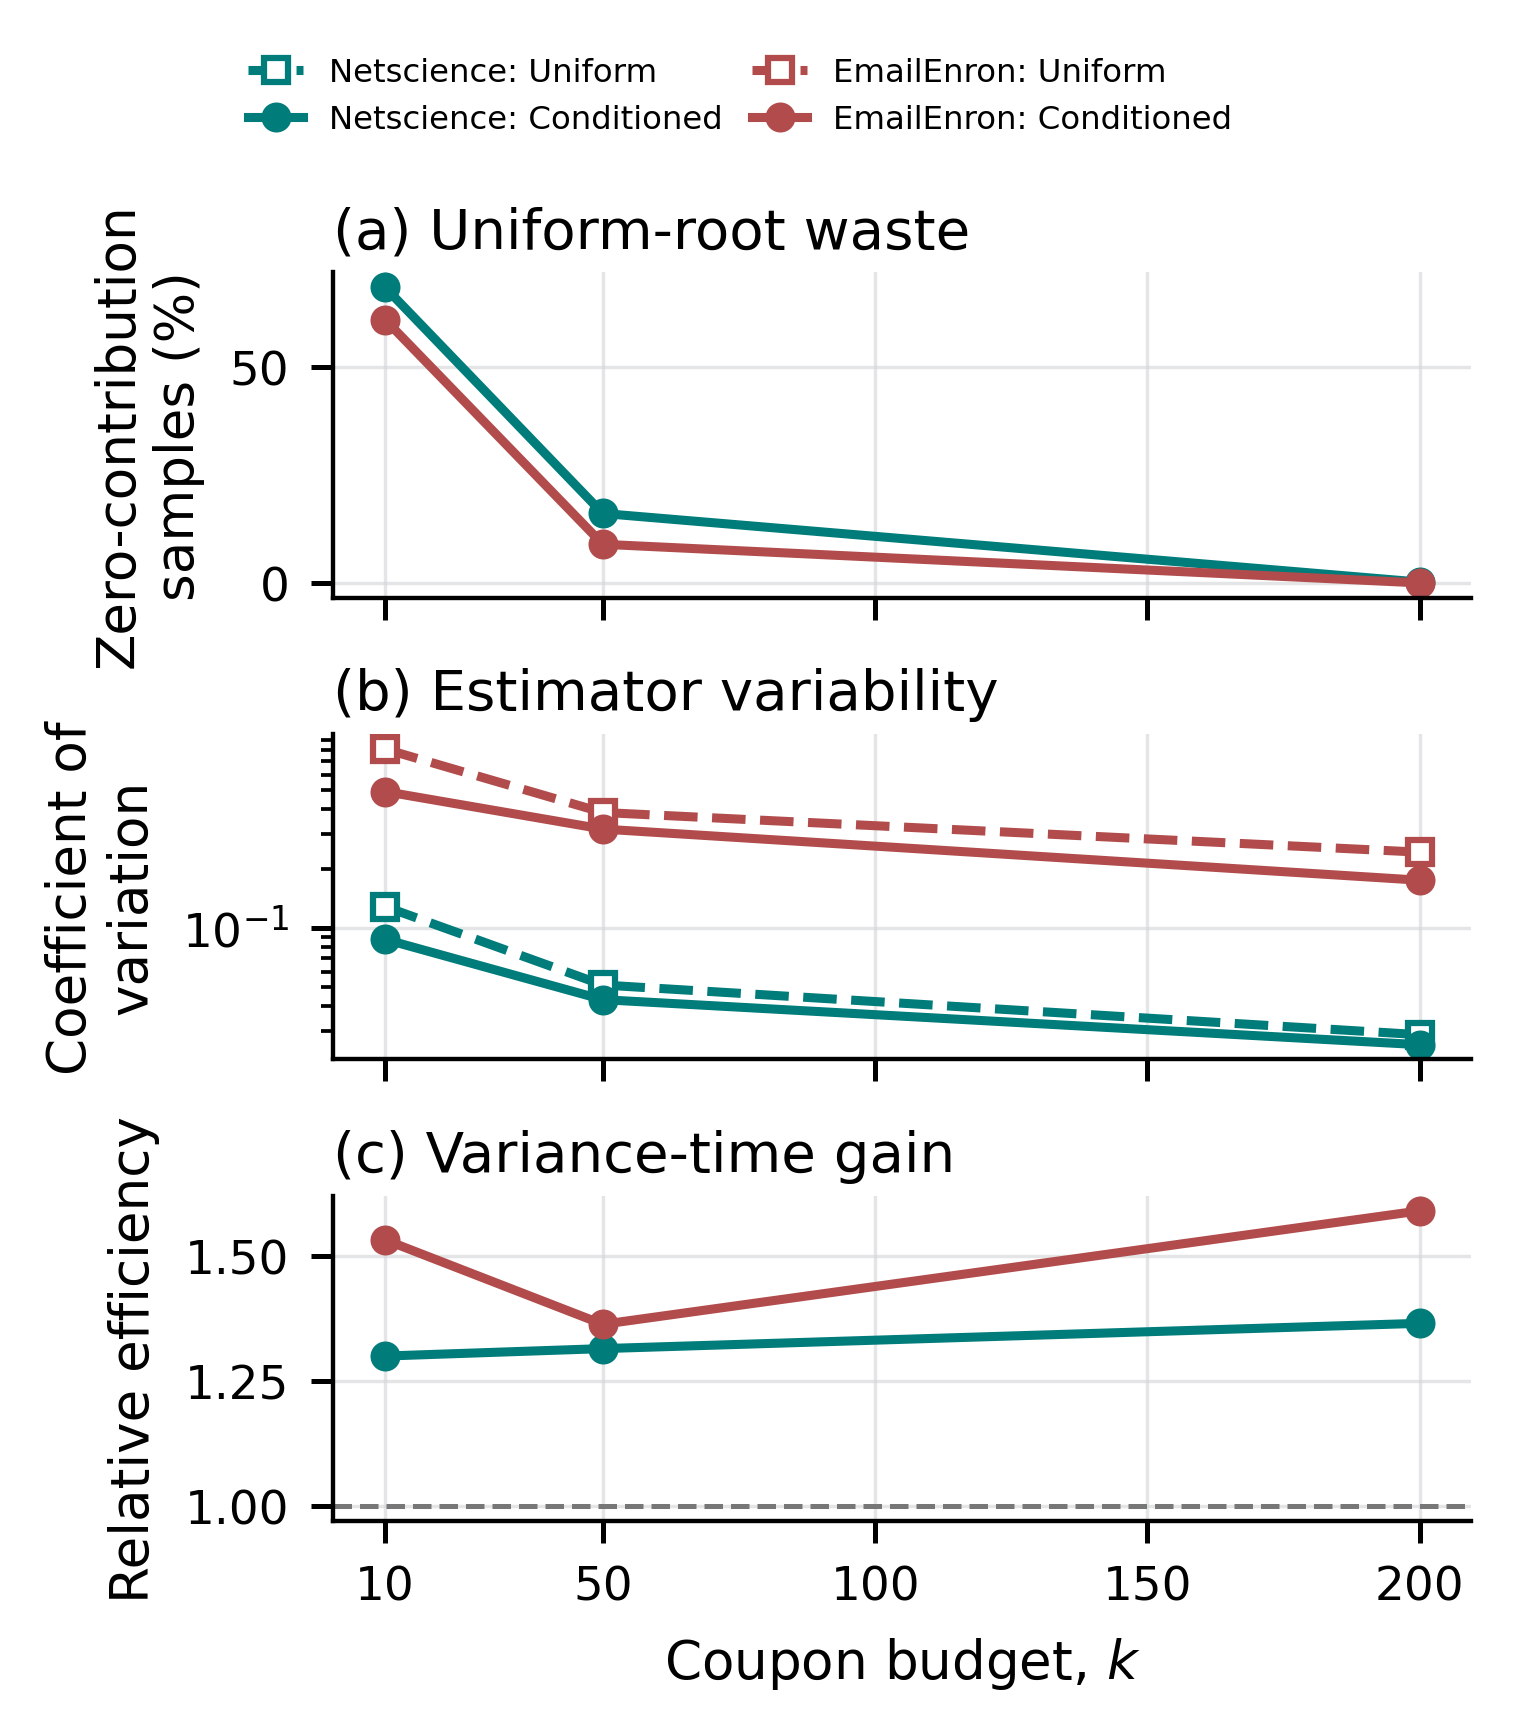
\includegraphics[width=\columnwidth]{figures/experiments/validated_sampler_ablation}
  \caption{Uniform-root versus conditioned-root estimation in the
  forwarding-heavy scenario. Each statistic uses 30 independent batches
  of $20{,}000$ samples. Relative efficiency is the ratio of the
  variance--time products of uniform and conditioned sampling; values
  above one favor conditioning.}
  \Description{Three panels compare zero-contribution samples,
  coefficient of variation, and variance-time efficiency for uniform and
  conditioned root sampling on Netscience and EmailEnron.}
  \label{fig:real-sampler}
\end{figure}

\begin{figure}[t]
  \centering
  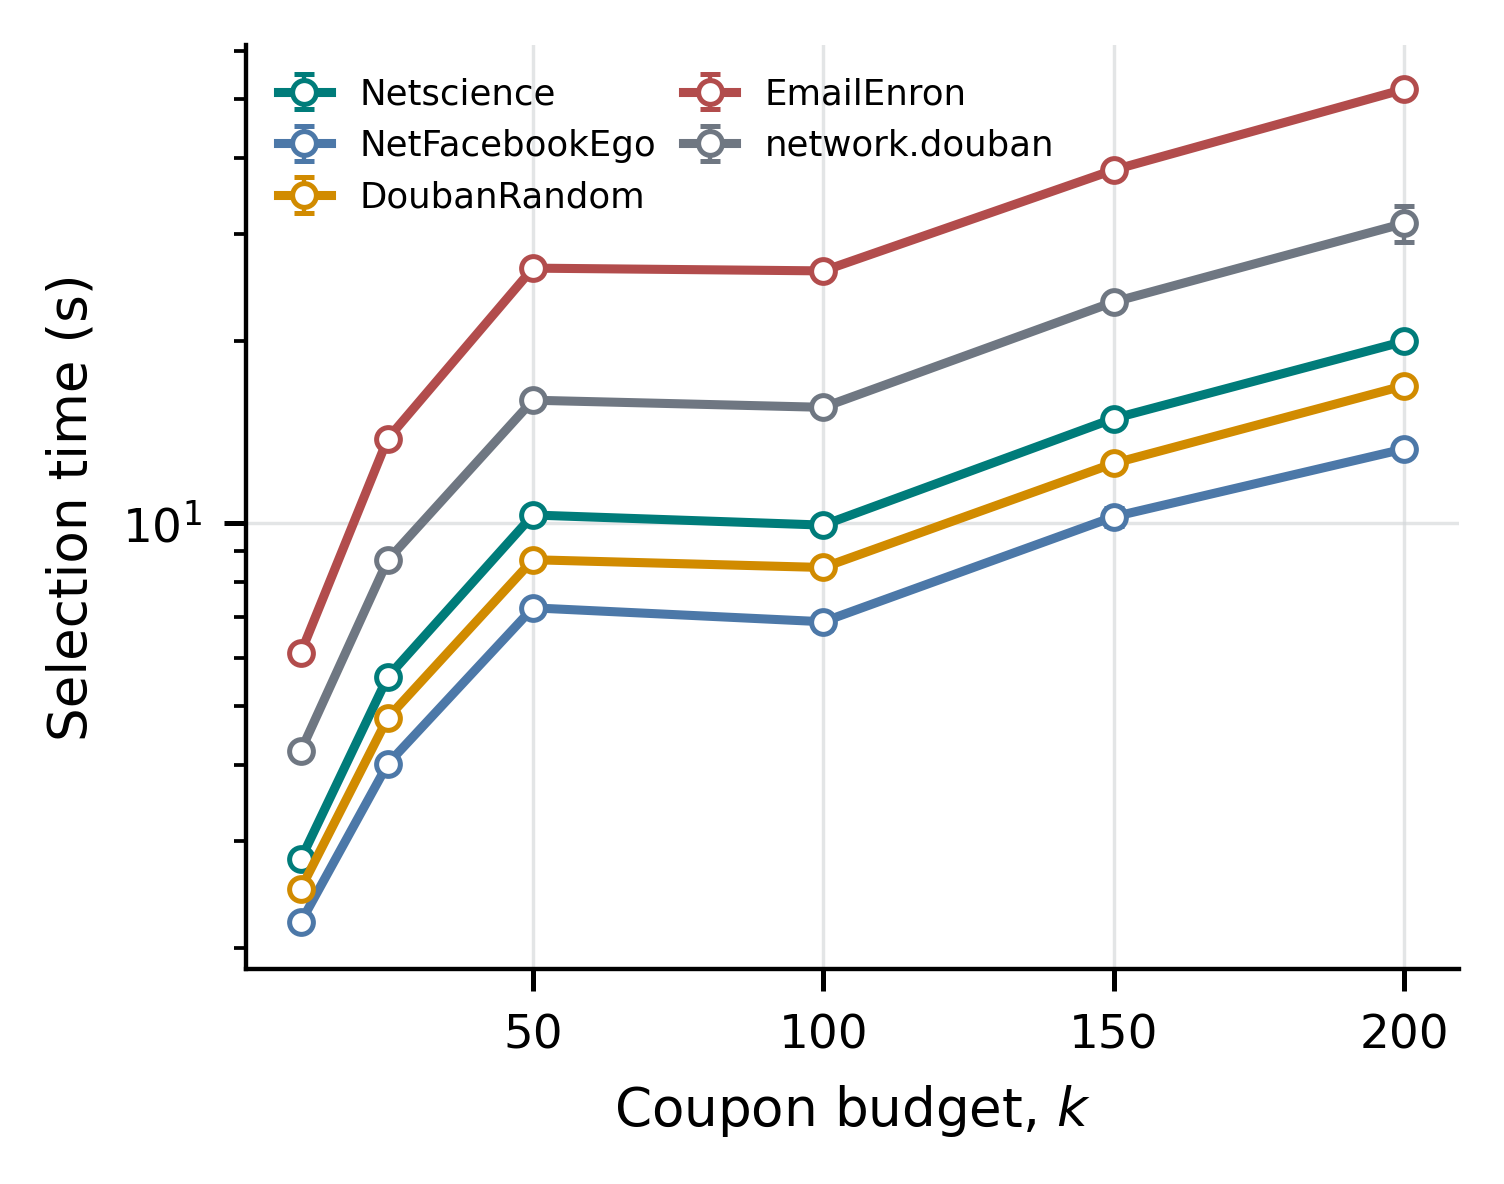
\includegraphics[width=\columnwidth]{figures/experiments/validated_runtime_scalability}
  \caption{Single-process \CIMRIS{} selection time in the balanced
  scenario, averaged over five runs. The sample budget is $100{,}000$ for
  $k\leq50$ and $50{,}000$ for $k\geq100$; error bars show one standard
  deviation.}
  \Description{A line chart plots selection time versus coupon budget
  for five graph instances on a logarithmic vertical scale.}
  \label{fig:real-runtime}
\end{figure}

Figure~\ref{fig:real-runtime} reports end-to-end \CIMRIS{} selection time,
including sample generation and greedy coverage.
The drop from $k=50$ to $k=100$ on several graphs is caused by the
pre-specified halving of the sample budget rather than a faster
per-sample computation.
At $k=200$, mean selection time is 51.9 seconds on EmailEnron and
31.2 seconds on
the larger network.douban graph.
The non-monotone ordering across real graphs reflects different degree
distributions and RR-set sizes; the result should therefore be read as
practical scalability evidence rather than a direct empirical fit of the
worst-case bound.

%% ============================================================
%% 7. CONCLUSION
%% ============================================================
\section{Conclusion}
\label{sec:conclusion}

We formalized coupon influence maximization under non-replicable,
single-path diffusion.
In this model, a coupon is redeemed, discarded, or transferred to one
neighbor, and only redemption creates an adopter.
The allocation formulation supports both distinct seeds and repeated
placements through per-node capacities while counting each adopter once.
We proved that CIM is NP-hard and that adoption spread is monotone and
DR-submodular over coupon allocations.
We then developed $k$-joint RR samples whose coverage gives unbiased
spread and marginal-gain estimates.
The resulting \CIMRIS{} algorithm achieves a
$(1-1/e-\epsilon)$ approximation with high probability and has expected
running time near-linear in the graph size when the budget, accuracy, and
spread lower bound are fixed.
Experiments show gaps of $0.3$--$11.1\%$ from high-precision Monte Carlo
greedy across two reference graphs and three scenarios; the largest gap
occurs for low-budget forwarding-heavy diffusion on NetFacebookEgo and
decreases as the RR sample budget grows.
Across all three scenarios, \CIMRIS{} outperforms DegreeTopM and PageRank at
every one of the 72 graph--budget pairs, with its largest average gains
appearing in the forwarding-heavy scenario.
Local and broadcast baselines remain competitive on some instances, so
no method dominates every graph and budget.
Conditioned root sampling removes zero-contribution samples and improves
the measured variance--time product by $1.3$--$1.5\times$ at $k=10$ on
the two tested graphs. Capacity experiments further show that repeated
placement provides a modest gain in the forwarding-heavy regime but is
rarely selected when adoption is common.

Several directions remain open.
First, extending the model to \emph{adaptive} allocation, where later
placements depend on observed early adoptions, could
reduce budget waste in time-sensitive campaigns.
Second, coupled campaign rules, such as one redemption per account or
forwarding incentives after adoption, require RR samples that encode
arrival order and user state.
Third, tighter lower-bound estimation and variance reduction for very
small adoption probabilities may further improve the practical cost of
\CIMRIS{}.

\appendix
\section{Additional Parameter-Regime Experiments}
\label{app:parameter-sweep}

The three scenarios in the main evaluation provide representative operating
points but do not show how the relative performance changes between them.
We therefore conduct a prespecified two-dimensional parameter sweep on
Netscience and NetFacebookEgo. This experiment is intended to map favorable
and unfavorable regimes rather than to establish that \CIMRIS{} dominates
every alternative.

Let $\hat d_u\in[0,1]$ be the normalized log-degree of node $u$. For a
central redemption share $r$ and transfer probability $t$, we set
\[
\begin{aligned}
  h_u &=
    \operatorname{clip}\!\left(r+0.20(0.5-\hat d_u),0.05,0.95\right),\\
  p_u^a&=(1-t)h_u,\qquad
  p_u^d=(1-t)(1-h_u),\qquad
  p_u^t=t.
\end{aligned}
\]
Thus $h_u$ controls the probability of redemption conditional on stopping,
while $t$ controls the expected persistence of a coupon walk. Transfer mass
is reassigned to discard at isolated nodes. The full grid uses
$t\in\{0.30,0.50,0.70,0.85,0.93\}$ and
$r\in\{0.20,0.40,0.60,0.80\}$ at $k=100$. We additionally fix $r=0.60$ and
evaluate $k\in\{25,100,200\}$ across all five transfer values. Every
configuration uses five selection seeds, $20{,}000$ samples for both
\CIMRIS{} and IC-RIS, and $2{,}000$ fresh forward realizations per allocation.
The comparison includes IC-RIS, 1Hop-Sort, Alpha-Sort, DegreeTopM, and
PageRank under the same distinct-seed policy. For each parameter cell, we
compare \CIMRIS{} with the baseline having the highest mean spread in that
cell; this is a stronger criterion than comparing against a fixed baseline.

\begin{figure*}[t]
  \centering
  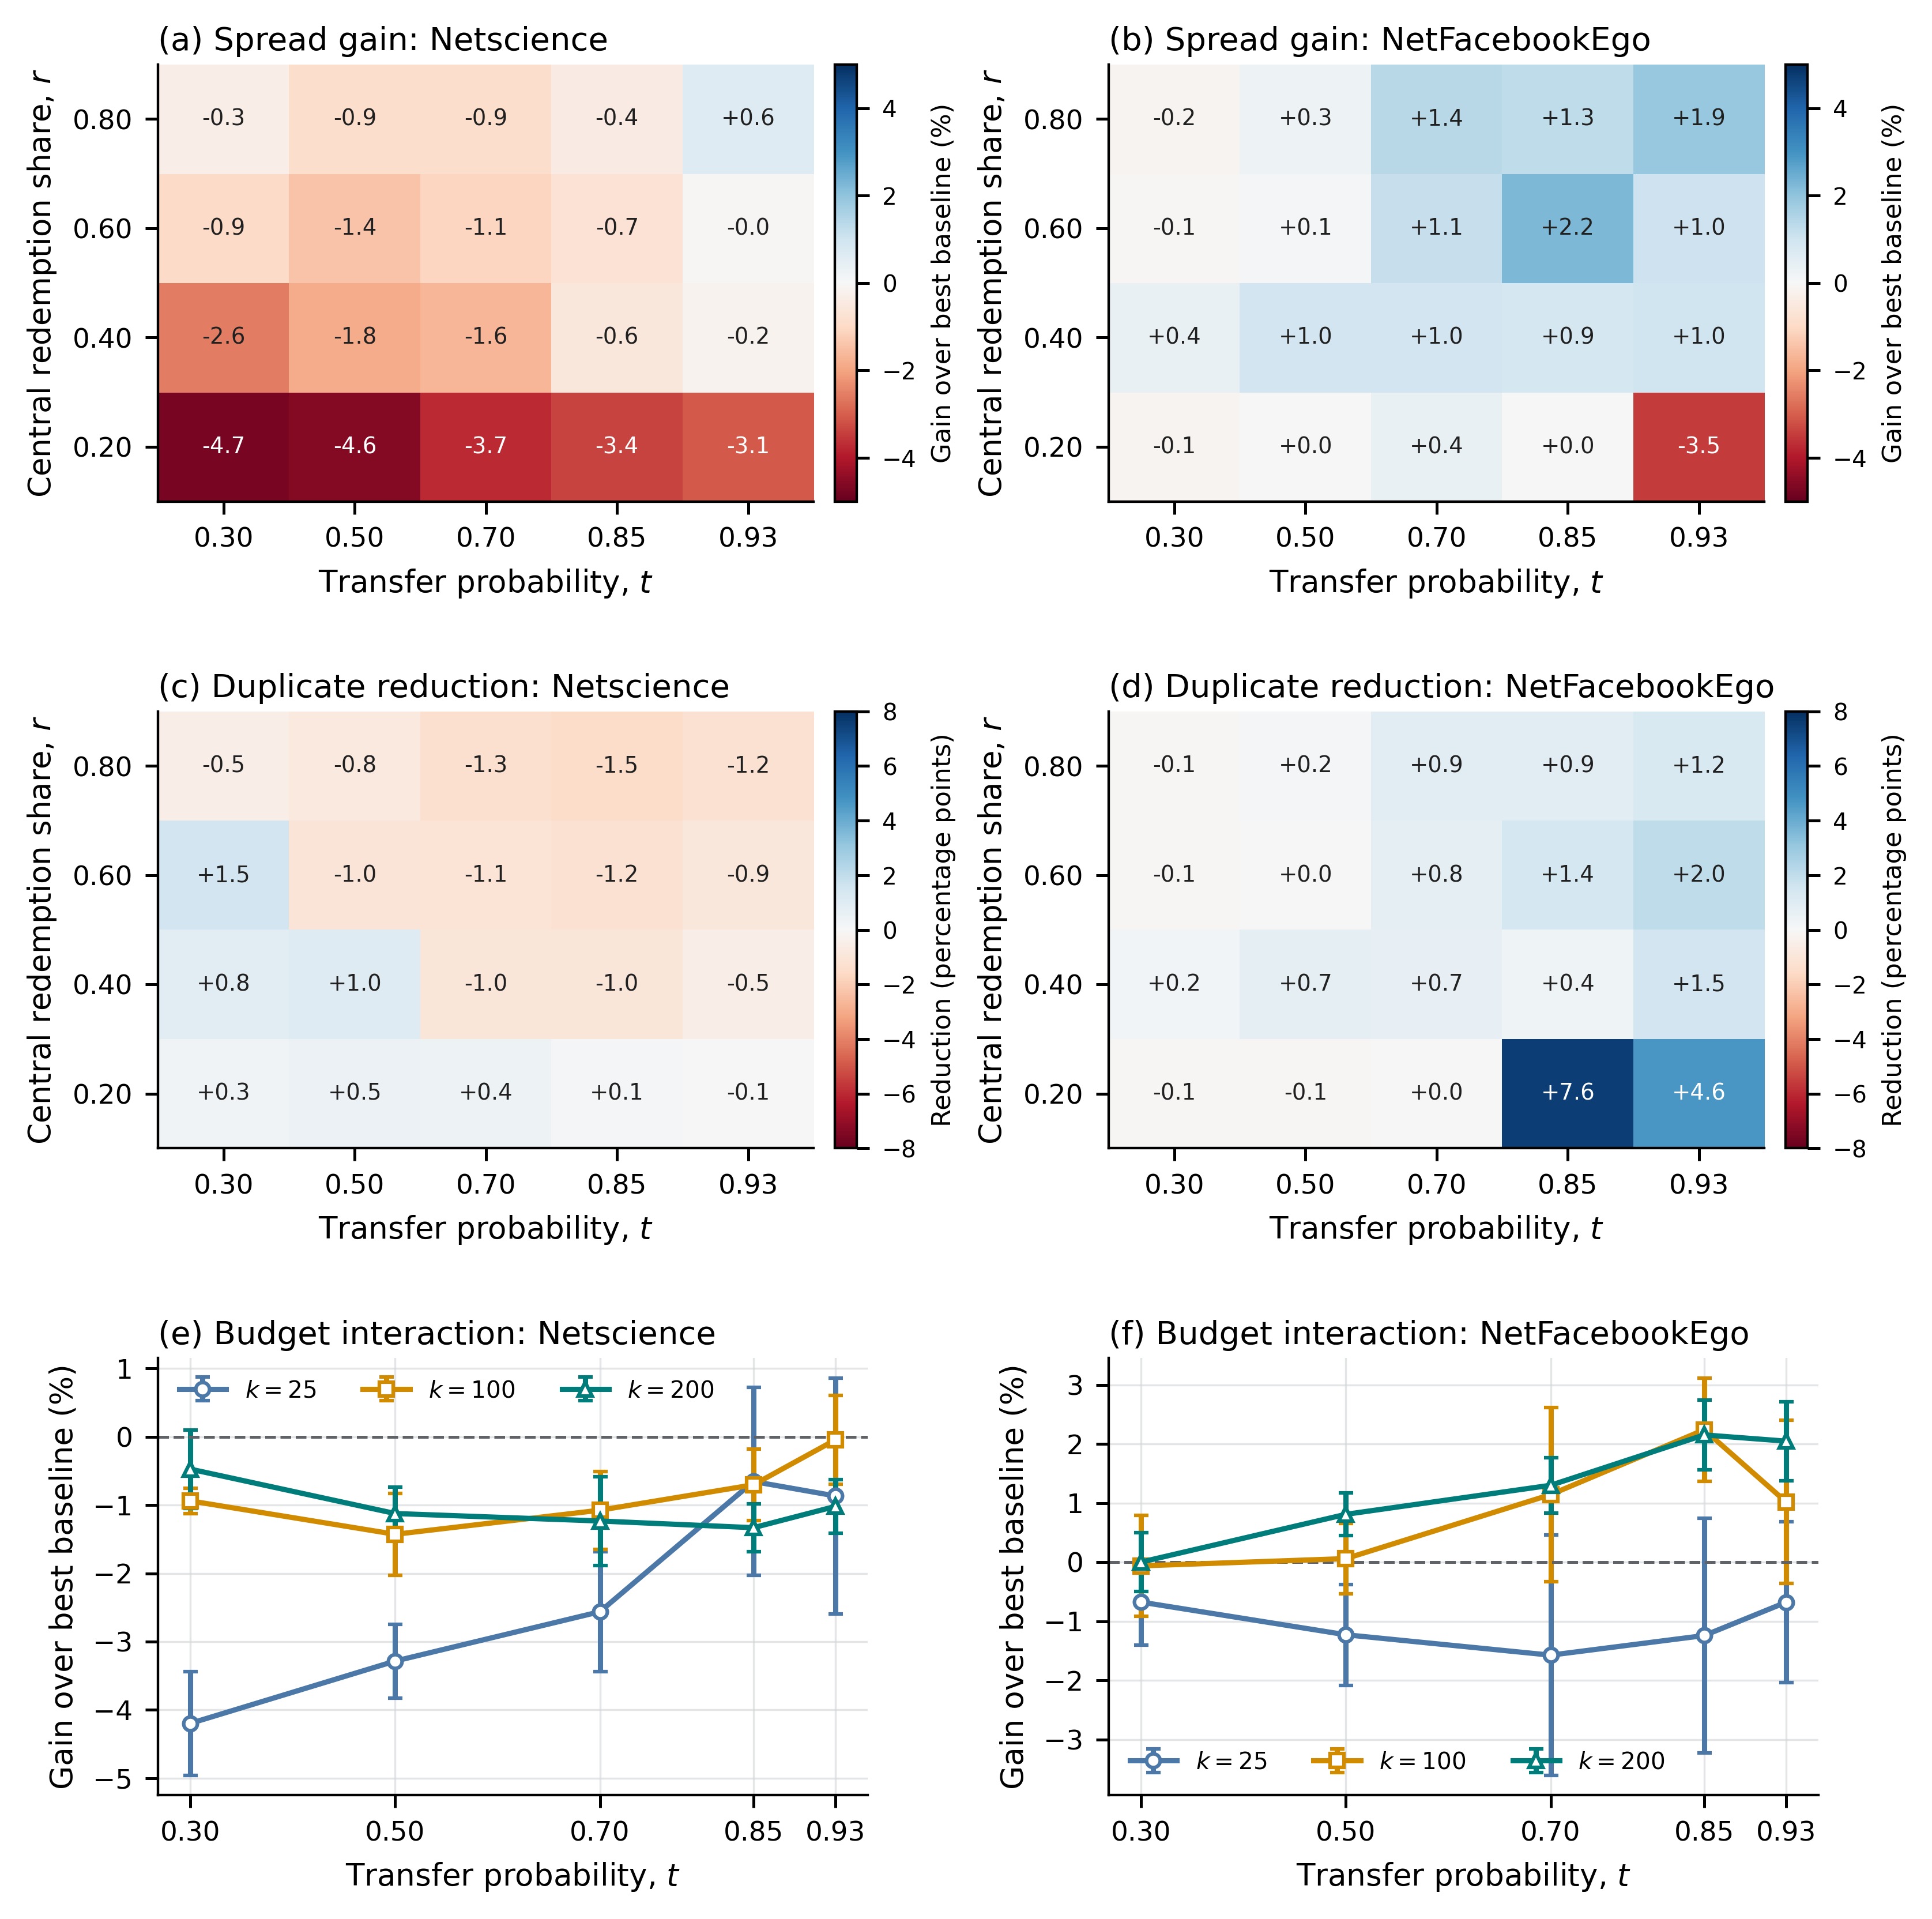
\includegraphics[width=0.96\textwidth]{figures/experiments/appendix_parameter_sweep}
  \caption{Complete parameter-regime study on two graph instances.
  (a--b) Relative adoption-spread difference between \CIMRIS{} and the
  strongest non-oracle baseline in each $k=100$ cell.
  (c--d) Reduction in duplicate-redemption fraction relative to that same
  baseline; positive values favor \CIMRIS{}.
  (e--f) Relative spread difference for $r=0.60$ as the budget changes.
  Heatmaps retain all prespecified cells, and line-chart error bars are
  95\% confidence intervals over five paired selection/evaluation runs.}
  \Description{Six panels report a complete transfer-probability by
  redemption-share parameter sweep. The first row shows spread gains over the
  strongest baseline, the second shows changes in duplicate-redemption
  fraction, and the third shows budget interactions on Netscience and
  NetFacebookEgo. Positive and negative regions are both visible.}
  \label{fig:appendix-parameter-sweep}
\end{figure*}

Figure~\ref{fig:appendix-parameter-sweep}(a--b) reports the complete $k=100$
grid. On NetFacebookEgo, \CIMRIS{} has higher mean spread than the strongest
baseline in 16 of 20 cells, with a mean relative difference of $0.50\%$ and a
maximum of $2.24\%$
at $(t,r)=(0.85,0.60)$. The exception at $(0.93,0.20)$ is substantial:
1Hop-Sort is $3.48\%$ higher. Netscience exhibits a different pattern:
\CIMRIS{} has higher mean spread in only one cell, has a mean difference of
$-1.62\%$, and ranges
from $-4.74\%$ to $0.63\%$. Nevertheless, it exceeds DegreeTopM and PageRank
in all 20 cells on both graphs. These results delimit the empirical advantage:
coupon-aware global coverage is most consistently useful on the larger,
sparser ego network, but it is not uniformly superior on the smaller
Netscience graph.

The budget slice in Figure~\ref{fig:appendix-parameter-sweep}(e--f) further
shows that the favorable region can depend on campaign scale. On
NetFacebookEgo, \CIMRIS{} has the higher mean in none of the five transfer
settings at $k=25$, four at $k=100$, and all five at $k=200$; the corresponding
mean differences are $-1.08\%$, $0.88\%$, and $1.26\%$. The same transition
does not occur on Netscience, where the strongest baseline retains the higher
mean at all three budgets throughout this slice.

Finally, Figure~\ref{fig:appendix-parameter-sweep}(c--d) compares the
duplicate-redemption fraction, defined as
$(\bar\rho-\bar\sigma)/\bar\rho$, with that of the strongest baseline.
Positive values indicate that \CIMRIS{} converts a larger fraction of
redemptions into distinct adopters. This quantity does not track spread gain
consistently: across the 40 cells at $k=100$, its Pearson correlation with the
relative spread difference is only $0.03$. Avoiding duplicate redemptions is
therefore one possible benefit of distinct-user coverage, but the measured
advantage also depends on whether an allocation reaches users who redeem at
all.
\FloatBarrier
\balance

\bibliographystyle{ACM-Reference-Format}
\bibliography{references}

\end{document}
